\chapter{Single particle motions and radiation mechanisms}
\label{Chap:Theory:SingleParticle}

This Chapter lays the theoretical groundwork for the results presented later in this work, addressing laser wakefield acceleration, radiation production from charged particles and the fundamental processes of radiation reaction and pair production.

Firstly, equation of motions of charged single particles in electromagnetic fields are derived. This forms the basis for understanding the properties of electrons accelerated in wakefield accelerators, measuring their energy in magnetic spectrometers and calculating the radiation they emit in interaction with electromagnetic fields.

Secondly, the propagation of a laser in a plasma and its non-linear evolution are discussed. This paves the way for the third section on laser wakefield acceleration where basic properties like maximum energy and injection mechanisms are introduced.

Subsequently, radiation production from electrons in different scenarios is discussed, starting with radiation in synchrotrons and insertion devices, then drawing the parallel to betatron radiation produced in wakefield acceleration and the radiation emitted in a laser wiggler, namely relativistic inverse Compton scattering (ICS) in moderately (linear ICS) and highly intense laser fields (non-linear ICS). Bremsstrahlung as radiation mechanism is also being introduced.

This leads over to the topic of radiation reaction, the knock-back force a charged particle experiences when emitting a photon. This can, for instance, be investigated in relativistic inverse Compton scattering. Whilst radiation reaction is a very fundamental phenomenon there is so far no universally accepted and practicable description for a wide parameter space. In this section different proposed descriptions of radiation reaction are discussed, starting with the in classical electrodynamics self-consistent Lorentz-Abraham-Dirac equation, followed by the classical Landau-Lifschitz equation and leading over to quantum corrections and their implications. 

Finally, other fundamental QED processes such as pair production, annihilation and light-light scattering is discussed.

\SMComm{Best way to structure: instead of many equations and long cross sections, try to find scaling laws in terms of relevant quantities of the experiment (yield, energy etc.). Move equations to appendix.}
\SMComm{Split theory in two parts.}
\EliasComm{Restructure appendix.}
\SMComm{Consider removing: cylindrical symmetry fields, axial, Debye length, plasma formation, quasi-neutrality.}
\SMComm{Consider dropping some wakefield stuff.}

\section{Single particle motion in an EM field}

The Lagrangian for a relativistic particle in an electromagnetic field with the potentials $\Phi$ and $\mathbf{A}$ is given by \cite{Jackson}
\begin{equation}
L(\mathbf{r},\mathbf{v},t) = - mc^2 \gamma^{-1}+q \mathbf{v}\cdot\mathbf{A} - q \Phi,
\end{equation}
where $m$ is the mass of the particle, $\gamma$ the relativistic Lorentz factor and $q$ the charge.
To obtain the equation of motion (EoM) we use the Euler-Lagrange equation
\begin{equation}
\frac{\mathrm{d}}{\mathrm{d}t} \frac{\partial L}{\partial \mathbf{v}} - \frac{\partial L}{\partial \mathbf{r}} = 0.
\end{equation}

Using $\mathbf{A} = \mathbf{A}(\mathbf{r},t)$, $\Phi = \Phi(\mathbf{r},t)$, $\gamma^{-1} = \sqrt{1-(v/c)^2}$ and this becomes
\begin{equation}
\frac{\mathrm{d}}{\mathrm{d}t} \left[\mathbf{p}+q\mathbf{A}\right]-\left[q\nabla\left( \mathbf{A} \cdot \mathbf{v}\right) - q\nabla \Phi \right] = 0,
\label{Theory:Eqns:EoMLorentzRaw}
\end{equation}
where $\mathbf{p} = \gamma m \mathbf{v}$ is the relativistic momentum.
Now using $\frac{\mathrm{d}}{\mathrm{d}t} = \frac{\partial}{\partial t} + \mathbf{v} \cdot \nabla$ and the vector identity $\nabla \left(\mathbf{v}\cdot\mathbf{A}\right) = (\mathbf{v}\cdot\nabla)\mathbf{A} + \mathbf{v}\times(\nabla\times\mathbf{A})$ this becomes:
\begin{equation}
\frac{\mathrm{d}}{\mathrm{d}t}\mathbf{p} = q\left(\mathbf{v} \times \nabla \times \mathbf{A}-\frac{\partial \mathbf{A}}{\partial t} - \nabla \Phi\right).
\label{Theory:Eqns:EoMLorentz}
\end{equation}

With the definitions of the electric field $\mathbf{E}$ and the magnetic field $\mathbf{B}$ in terms of the potentials  $\Phi$ and $\mathbf{A}$
\begin{align}
\mathbf{E} &= -\frac{\partial \mathbf{A}}{\partial t} - \nabla \Phi,\\
\mathbf{B} &= \nabla \times \mathbf{A},
\end{align}

the equation of motion takes the familiar shape of the Lorentz force:

\begin{equation}
\boxed{\frac{\mathrm{d}\mathbf{p}}{\mathrm{d}t} = q \left(\mathbf{E} + \mathbf{v} \times \mathbf{B}\right).}
\end{equation}

\subsection{Electron motion in a homogeneous electric field}

Using the previously derived equation for the Lorentz force we can now consider a first simple example. Consider the motion of a single electron in a homogeneous electric field without presence of a magnetic field, i.e. $\mathbf{B} = \mathbf{0}$. The Lorentz equation simplifies to:

\begin{equation}
\frac{\mathrm{d}\mathbf{p}}{\mathrm{d}t} = q \mathbf{E}.
\end{equation}

If we choose the coordinate system such that  $\mathbf{E} =  (E,0,0)^t = E e_x$, we see that the momentum of the electron is unchanged in the other two directions, $\mathrm{d}p_x/\mathrm{d}t = \mathrm{d}p_y/\mathrm{d}t = 0$. In x-direction the electron however feels a constant force $qE$ accelerating it at a linear energy gain.

\subsection{Electron motion in a homogeneous magnetic field}

Consider the motion of a single electron in a homogeneous magnetic field extending over the entire region of interest. The equation for the Lorentz force simplifies with $\mathbf{E} = \mathbf{0}$ to:
\begin{subequations}
\begin{align}
\frac{\mathrm{d}\mathbf{p}}{\mathrm{d}t} &= q \mathbf{v} \times \mathbf{B},\\
\frac{\mathrm{d}\mathbf{p}}{\mathrm{d}t} &= \frac{q}{\gamma m} \mathbf{p} \times \mathbf{B},
\end{align}
\end{subequations}
in terms of the relativistic momentum $\mathbf{p} = \gamma m \mathbf{v}$.
Note that in this case the purely magnetic Lorentz force does not do any work. The instantaneous rate of work (power) is $P = \mathbf{F} \cdot \mathbf{v}$, where the force $\mathbf{F}$ is by virtue of the cross product always orthogonal to $\mathbf{v}$ and the dot product vanishes.
We choose the coordinate system such that $\mathbf{B} = (0,0,B)^t = B e_z$. The momentum vector is simply $\mathbf{p} = (p_x,p_y,p_z)^t$.
The differential equations are then given by:
\begin{subequations}
\begin{align}
\dot{p_x} &= \frac{qB}{\gamma m} p_y,\\
\dot{p_y} &= - \frac{qB}{\gamma m} p_x,\\
\dot{p_z} &= 0,
\end{align}
\end{subequations}
which combines to
\begin{subequations}
\begin{align}
\ddot{p_x}  &= - \left(\frac{qB}{\gamma m}\right)^2 p_x,\\
\ddot{p_y}  &= - \left(\frac{qB}{\gamma m}\right)^2 p_y.
\end{align}
\end{subequations}
This second order, linear differential equation can be solved by a periodic motion of type $p_x(t) = C \sin(\omega t) + D \cos(\omega t)$ with $\omega = qB/\gamma m$. The dotted variables indicate the time derivatives with $\dot{p} = \mathrm{d}p/\mathrm{d}t$ and $\ddot{p}=\mathrm{d}^2p/\mathrm{d}^2t$.

$\mathbf{p_\perp}$ be the momentum vector of the particle perpendicular to the magnetic field lines and $\mathbf{p_\parallel}$ the component parallel to the magnetic field (z). For the initial conditions $p_x(t=0) = |\mathbf{p_\perp}| = p_\perp$ and $p_y(t=0)=0$, we obtain for the momenta:
\begin{subequations}
\begin{align}
p_x(t) &= p_\perp \cos(\omega t)\\
p_y(t) &= - p_\perp \sin(\omega t) 
\end{align}
\end{subequations}
The solution for the z-motion is trivial with $p_z = p_{z,0}$.
Expressed in terms of the trajectories with initial conditions $x(0) = 0, z(0) = 0, y(0) = p_\perp/qB = r_{L}$, this reads
\begin{subequations}
\begin{empheq}[box=\widefbox]{align}
x(t) &= r_{L} \sin(\omega t)\\
y(t) &= r_{L} \cos(\omega t)\\
z(t) &= \frac{p_{z,0}}{\gamma m} t
\end{empheq}
\end{subequations}

The radius of the circular motion of the electron is called the Larmor radius $r_L$. It depends on the total momentum in the x-y plane and the magnetic field strength $B$: 
\begin{equation}
\boxed{r_{L} = |\mathbf{p}_\perp|/eB,}
\end{equation}
where $e$ is the charge of the electron and $\mathbf{p}_\perp$ is the component of the momentum vector $\mathbf{p}$ that is perpendicular to the field component of the magnetic field.
\vspace{\baselineskip}

The motion of the electron consists of two decoupled motions: one at the constant, initial velocity parallel to the magnetic field vector in $z$, the second motion is a circular motion in the x-y plane. This is called a cyclotron motion. For now we will ignore the dissipation of energy in form of radiation due to the acceleration of the electron and accept the result that the Lorentz force conserves the total momentum and energy of the particle in this case.

\subsection{Electron motion in a monochromatic plane EM wave}
\label{Theory:Sec:SingleParticle:FigOfEight}

Writing the equation of motion in terms of the potentials $\mathbf{A}$ and $\Phi$ as in Equation \eqref{Theory:Eqns:EoMLorentz} on page \pageref{Theory:Eqns:EoMLorentz} gives \cite{ThomasThesis}:

\begin{equation}
\frac{\mathrm{d}}{\mathrm{d}t}\mathbf{p} = q\left(\mathbf{v} \times \nabla \times \mathbf{A}-\frac{\partial \mathbf{A}}{\partial t} - \nabla \Phi\right).
\end{equation}

Now using the convective derivative and the vector identity $\mathbf{v} \cdot \nabla \mathbf{p} = (\nabla \mathbf{p})\cdot\mathbf{v} - \mathbf{v} \times (\nabla\times\mathbf{p})$ again, the total time derivative of the momentum expands to
\begin{equation}
\frac{\mathrm{d}}{\mathrm{d}t}\mathbf{p} = \frac{\partial\mathbf{p}}{\partial t} +(\nabla\mathbf{p})\cdot\mathbf{v} - \mathbf{v}\times(\nabla\times\mathbf{p}).
\end{equation}
\EliasComm{Add derivation to Appendix for vector identity.}
With this result the equation of motion becomes
\begin{align}
\frac{\partial\mathbf{p}}{\partial t} +(\nabla\mathbf{p})\cdot\mathbf{v} - \mathbf{v}\times(\nabla\times\mathbf{p}) &= q\left(\mathbf{v} \times \nabla \times \mathbf{A}-\frac{\partial \mathbf{A}}{\partial t} - \nabla \Phi\right),\nonumber\\
\frac{\partial}{\partial t}\left(\mathbf{p}+q\mathbf{A}\right) +(\nabla\mathbf{p})\cdot\mathbf{v} - \mathbf{v}\times\left(\nabla\times\left(\mathbf{p}+q\mathbf{A}\right)\right) &= - q\nabla \Phi,\nonumber\\
\frac{\partial}{\partial t}\mathbf{u} +(\nabla\mathbf{p})\cdot\mathbf{v} - \mathbf{v}\times\left(\nabla\times\mathbf{u}\right) &= - q\nabla \Phi,
\label{Theory:Eqns:EoMLaserAT}
\end{align}
where we introduced in the last step the canonical momentum $\mathbf{u} = \mathbf{p} + q\mathbf{A}$.
We can express $(\nabla\mathbf{p})\cdot \mathbf{v}$ as follows
\begin{equation}
(\nabla\mathbf{p})\cdot \mathbf{v} = \frac{1}{m\gamma} \nabla (p^2/2) = \frac{1}{m\gamma}\nabla(\gamma^2/2) = m c^2 \nabla \gamma.
\label{Theory:Eqns:nablaDotV}
\end{equation}

Substituting $(\nabla\mathbf{p})\cdot \mathbf{v}$ in Equation \eqref{Theory:Eqns:EoMLaserAT} by the expression in Equation \eqref{Theory:Eqns:nablaDotV}:
\begin{equation}
\frac{\partial}{\partial t}\mathbf{u} = \mathbf{v}\times\left(\nabla\times\mathbf{u}\right) - \nabla \left(q\Phi + \gamma mc^2\right).
\label{Theory:Eqns:partialtU}
\end{equation}

Taking the curl of this equation results in:
\begin{equation}
\frac{\partial}{\partial t}\nabla\times\mathbf{u} = \nabla\times\left[\mathbf{v}\times\left(\nabla\times\mathbf{u}\right)\right],
\end{equation}
where the second term disappeared as the curl of a gradient is always zero (see Section \ref{Appendix:VectorIdentities:CurlGradZero}),
so that if $\nabla \times \mathbf{u}$ is zero initially, it will remain so always. The condition is satisfied, for instance, for a plasma at rest before the laser pulse arrives.
Assuming this condition Equation \eqref{Theory:Eqns:partialtU} simplifies to
\begin{equation}
\frac{\partial}{\partial t}\mathbf{u} = - \nabla \left(q\Phi + \gamma mc^2\right).
\end{equation}

For a medium close to vacuum or an unperturbed plasma one can assume $\Phi = 0$, resulting in:
\begin{equation}
\frac{\partial}{\partial t}\mathbf{u} =  -\nabla\gamma mc^2.
\end{equation}
In the case of an infinite plane wave the transverse gradient $\nabla_\perp$ is zero.
This means we obtain two separate components:
\begin{subequations}
\begin{align}
\frac{\partial}{\partial t}\mathbf{u}_\perp &= 0,\\
\frac{\partial}{\partial t}\mathbf{u}_\parallel &= \nabla_\parallel \gamma mc^2.
\end{align}
\end{subequations}

From the perpendicular component we see that the transverse canonical momentum is conserved: $\mathbf{p}_\perp + q\mathbf{A} = 0$. If $q = -e$ and $e\mathbf{A}_\perp = \mathbf{a}_\perp$, then $\mathbf{p}_\perp = \mathbf{a}_\perp$. In Cartesian coordinates, this means $p_x = a_x, p_y = a_y$.

For the parallel spatial component $z$ consider the substitution $z = ct$ for light. Thus, $\partial z = c \partial t$. The parallel-component of the vector potential $\mathbf{A}$ is zero, so $u_\parallel = p_\parallel = p_z$:

\begin{equation}
\frac{\partial}{\partial t}(cp_z - \gamma mc^2) = 0.
\end{equation}

Assuming an unperturbed stationary plasma, the initial conditions are $\gamma(t=0) = 1$ and $p_z(t=0) = 0$. Integrating the previous equation gives:
\begin{equation}
c p_z+ mc^2 = \gamma mc^2.
\end{equation}

Using $E = \gamma m c^2 = \sqrt{mc^2 + (cp_\parallel)^2 + (cp_\perp)^2}$ and substituting, one obtains an expression for $p_\parallel = p_z$:

\begin{equation}
p_z = \frac{1}{2} mc a^2,
\end{equation}
where $a^2 = p^2_\perp$.
We now have
\begin{subequations}
\begin{align}
p_x &= mc a_x,\\
p_y &= mc a_y,\\
p_z &= \frac{1}{2} mc a^2.
\end{align}
\end{subequations}

Using $\mathbf{p} = \gamma m \mathbf{v}$ this can be written as:
\begin{subequations}
\begin{align}
\frac{\gamma}{c} \frac{\mathrm{d}x}{\mathrm{d}t} &= a_x,\\
\frac{\gamma}{c} \frac{\mathrm{d}y}{\mathrm{d}t} &= a_y,\\
\frac{\gamma}{c} \frac{\mathrm{d}z}{\mathrm{d}t} &= \frac{a^2}{2}.
\end{align}
\end{subequations}

Changing from $t$ to proper time $\tau$, we transform via $\mathrm{d}\tau = \gamma^{-1}\mathrm{d}t$, simply giving the equation of motions in term of $\tau$:
\begin{subequations}
\begin{align}
\frac{1}{c}\frac{\mathrm{d}x}{\mathrm{d}\tau} &= a_x,\\
\frac{1}{c}\frac{\mathrm{d}y}{\mathrm{d}\tau} &= a_y,\\
\frac{1}{c}\frac{\mathrm{d}z}{\mathrm{d}\tau} &= \frac{a^2}{2}.
\end{align}
\end{subequations}

Let us assume a laser field with linear polarisation in $x$, described by the vector potential
\begin{equation}
\mathbf{a} = a_0 \cos(kz - \omega t)\mathbf{e}_x = a_0 \cos(\xi)\mathbf{e}_x,
\end{equation}
where $\mathbf{e}_x$ is the unit vector in the x-coordinate, $\xi = kz - \omega t$ the waveframe coordinate and $k = \omega/c$ the wave number. 

\begin{figure}[h]
\centering
	\includegraphics[width=0.49\columnwidth]{figeight_lab.pdf}
	\includegraphics[width=0.49\columnwidth]{figeight_drift.pdf}
\caption[Electron motion in an infinite, linearly polarised, plane EM wave.]{Electron motion in an infinite, linearly polarised, plane EM wave in the lab frame (left), with the wavenumber $k = \omega/c$. On the right the figure-of-eight motion in the drift frame.}
\label{Theory:Figs:FigureOfEight}
\end{figure}

Using this explicit vector potential:
\begin{subequations}
\begin{align}
\frac{\gamma}{c}\frac{\mathrm{d}x}{\mathrm{d}t} &= a_0 \cos \xi,\\
\frac{\gamma}{c}\frac{\mathrm{d}y}{\mathrm{d}t} &= 0,\\
\frac{\gamma}{c}\frac{\mathrm{d}z}{\mathrm{d}t} &= \frac{1}{2} a^2_0 \cos^2 \xi.
\end{align}
\end{subequations}

and integrating the equation of motions, results in:
\begin{subequations}
\begin{align}
x(\xi) &= \frac{a_0}{k}\sin(\xi),\\
y(\xi) &= 0,\\
z(\xi) &= \frac{a^2_0}{4k}\left(\xi + \frac{1}{2}\sin(2\xi)\right),
\end{align}
\end{subequations}
where we chose the initial conditions $x(0)=y(0)=z(0)=0$  and used $\mathrm{d}\xi/\mathrm{d}t = \omega/\gamma$.

The electron is performing a periodic oscillation around the z-axis, whilst the motion in the z-axis is composed of a constant drift and another oscillation (see Figure \ref{Theory:Figs:FigureOfEight} (left)). This is commonly referred to as the `figure-of-eight' motion, which becomes more evident in the drift frame (see Figure \ref{Theory:Figs:FigureOfEight} (right)). For $a_0 \leq 1$ the motion in z is suppressed and the motion of the electron is dominated by the transverse oscillation. For $a_0 \gg 1$, the motion is predominantly longitudinal.



\subsection{Electron in a cylindrically symmetric electric field}

The previously discussed case of a particle in a homogeneous magnetic field corresponds to the motion in a magnetic electron spectrometer or the deflection of charged particles in a circular accelerator.
We will now discuss the motion of an electron in a cylindrically symmetric electric field which resembles the case of an electron in a plasma channel.
This derivation is based on \cite{WoodThesis}.

Assume a relativistic electron moving in the longitudinal direction and an electric field that is cylindrically symmetric around the propagation axis.
We ignore any vector potential contributions and only use a scalar potential.
The Lagrangian of this scenario is described by
\begin{equation}
L(\mathbf{r},\mathbf{v},t) = - m_e c^2 \gamma^{-1} - q \Phi,
\end{equation}
where $\Phi$ is the scalar potential describing the electrostatic field of the channel.
The scalar potential is the solution matching the radial Poisson equation in cylindrical symmetry

\begin{equation}
\frac{1}{r} \frac{\partial}{\partial r} \left(r \frac{\partial \phi}{\partial r}\right) = \frac{- e (n_0 - n_e)}{\epsilon_0},
\end{equation}

with the solution 
\begin{equation}
\phi = -\frac{(n_0 - n_e) e r^2}{4 \epsilon_0},
\end{equation}
where $n_0$ is the ion charge density and $n_e$ the electron density in the channel. 
In the limit of a completely evacuated channel, $n_e \rightarrow 0$, $\phi = -n_0 er^2/(4\epsilon_0)$.
As before $\mathbf{E} = - \nabla \phi$ and in this case $E_r = - \partial_r \phi$.
The equation of motion for the radial component is then
\begin{equation}
\frac{d}{dt} \mathbf{p} = - \frac{e^2 n_0}{2 \epsilon_0} r,
\end{equation}
with $\mathbf{p} = \gamma m_e \mathbf{\dot{r}}$.
Assume there is no axial acceleration field, the radial component of the velocity is small compared to $c$ and the longitudinal component is close to $c$: $\dot{\gamma}$ is then close to zero. 
The equation then takes the shape of a harmonic oscillator
\begin{equation}
\ddot{r} = - \frac{e^2 n_0}{2\epsilon_0 m_e \gamma} r = - \omega_\beta^2 r,
\end{equation}

with a frequency we will call the betatron frequency, $\omega_\beta$, which is related to the plasma frequency, $\omega_p$, by $\omega_\beta = \omega_p/\sqrt{2\gamma}$. The plasma frequency will be derived explicitly in Section \ref{Chap:Theory:Sec:PlasmaFreq}.
As this is the standard harmonic oscillator equation, it follows a solution of shape
\begin{equation}
r(t) = A \cos (\omega_\beta t + \varphi),
\end{equation}
and with initial conditions $r(t=0) = r_\beta$ and $\dot{r}(t=0) = 0$, we obtain
\begin{equation}
r(t) = r_\beta \cos(\omega_\beta t),
\end{equation}
where $r_\beta$ is the amplitude of the oscillation, also referred to as the betatron radius.
\vspace{\baselineskip}

If we continue with the assumption $\dot{\gamma} = 0$, this requires $\beta^2 = \beta^2_r + \beta^2_z = constant$. This gives $\beta_z = \sqrt{\beta^2 - \beta^2_r} \approx \beta (1-\beta^2/2)$, where we used a Taylor expansion and $\beta \approx 1$. If we use the solution for $r(t)$ derived above, $\beta_r = \dot{r}/c$ and $\sin^2 x = (1-\cos 2\theta)/2$, we obtain:
\begin{equation}
\beta_z \approx \beta \left(1-\frac{r^2_\beta \omega^2_\beta}{4 c^2}\right) + \beta \frac{r^2_\beta \omega^2_\beta}{4c^2} \cos (2 \omega_\beta t).
\end{equation}

Integrating this with the initial condition $z(t=0) = z_0$

\begin{equation}
\frac{z}{c} \approx \frac{z_0}{c} + \beta \left(1-\frac{r^2_\beta \omega^2_\beta}{4 c^2}\right) t + \beta \frac{r^2_\beta \omega_\beta}{8c^2}\sin(2\omega_\beta t),
\end{equation}

where we identify the drift velocity $\beta c \left(1-\frac{r^2_\beta \omega^2_\beta}{4 c^2}\right)$ and in the moving frame the familiar figure-of-eight motion again.


\subsection{Electron in a cylindrically symmetric electric field with axial field}

Now we add will add a constant axial field in the longitudinal (direction of electron propagation) to the previous case. This comes closer to the reality of a laser wakefield accelerator where electrons experience radial focusing and axial accelerating fields at the same time. Significant parts of this derivation are based on \cite{WoodThesis,Glinec2008_BETATRON}.

The electric field component shall now be $E_z$, with $z$ being the longitudinal axis.
This gives us the extra term $\frac{\partial \phi}{\partial z} = - E_z$.
The Euler-Lagrangian now has two non-trivial equations of motions.
First, as before
\begin{equation}
\frac{d}{dt} (\gamma m_e \dot{r}) = \frac{\partial }{\partial r} L = -\frac{e^2 n_0}{2\epsilon_0} r,
\label{Theory:Eq:EoM_Rad_Ax_R}
\end{equation}
and, second, the z-component
\begin{equation}
\frac{d}{dt} (\gamma m_e \dot{z}) = \frac{\partial }{\partial z} L = e E_z = const.
\label{Theory:Eq:EoM_Rad_Ax_Z}
\end{equation}

The change in momentum is now not negligible any more, $\dot{\gamma}\neq 0$, and we have to expand the brackets on the left-hand side of Equations \eqref{Theory:Eq:EoM_Rad_Ax_R} and \eqref{Theory:Eq:EoM_Rad_Ax_Z}.
The radial component is then
\begin{equation}
\dot{\gamma}m_e \dot{r} + \gamma m_e \ddot{r} = - \frac{e^2 n_0}{2 \epsilon_0} r.
\end{equation}

The axial component is equal to a constant, so we can simply integrate
\begin{equation}
\gamma m_e \dot{z} = - e E_z t + const.
\end{equation}

If we assume that the electron is highly relativistic $\dot{z} \rightarrow c$, so $\dot{\gamma} = eE_z/m_e c$ and

\begin{equation}
\gamma \beta_z \approx \gamma = - \frac{e E_z t}{m_e c} + \gamma_0 \beta_0,
\label{Theory:Eq:EoM_Rad_Ax_Gamma}
\end{equation}

where $\gamma_0 \beta_0$ are the initial conditions.
\begin{figure}
\centering
\includegraphics[width=.8\columnwidth]{betatron_traj.pdf}
\caption[Particle trajectory of an electron in a cylindrically symmetric electric field with a constant axial accelerating field.]{Particle trajectory of an electron in a cylindrically symmetric electric field with a constant axial accelerating field as described in Equation \eqref{Theory:Eqs:EoM_Betatron} for a plasma of density $n_e = 2 \times 10^{18} cm^{-3}$ as a function of propagation distance.}
\label{Theory:Figs:BetatronMotion}
\end{figure}
Inserting the result from Equation \eqref{Theory:Eq:EoM_Rad_Ax_Gamma} into Equation \eqref{Theory:Eq:EoM_Rad_Ax_R}, we obtain the differential equation

\begin{equation}
eE_z \dot{r} + (eE_z t + \gamma_0 \beta_0 m_e c) \ddot{r} = - \frac{e^2 n_0 c}{2 \epsilon_0} r,
\end{equation}
which we can write as 
\begin{equation}
(At + B) \ddot{r} + A \dot{r} + C r = 0,
\end{equation}
by using the abbreviations $A = eE_z$, $B = \gamma_0 \beta_0 m_e c$ and $C = e^2 n_0 c/2\epsilon_0$.
The analytic solution for this differential equation is:
\begin{subequations}
\begin{empheq}[box=\widefbox]{align}
r(t) = \frac{\pi \sqrt{CB}}{A} r_{\beta 0} \Biggl[ &J_1 \left( 2 \sqrt{CB}/A \right) Y_0 \left(2 \sqrt{C (B+At)}/A\right) \\  \nonumber
&- Y_1 \left(2\sqrt{CB}/A\right)J_0\left(2\sqrt{C(B+At)}/A\right)\Biggr],
\end{empheq}
\label{Theory:Eqs:EoM_Betatron}
\end{subequations}
with the initial conditions $r(t=0) = r_{\beta 0}$ and $\dot{r}(t=0) = 0$. $J_1, J_0$ are Bessel functions of first kind of order $1$ and $0$, respectively. $Y_1, Y_0$ are Bessel function of the second kind of order $1$ and $0$.
This motion is shown in Figure \ref{Theory:Figs:BetatronMotion}. We see that the oscillations quickly lose amplitude and fall to a settled value, whereas the wavelength of the oscillations increases as the electron gains momentum and inertia.

\subsection{Ponderomotive Force}

In laser wakefield acceleration (LWFA) a high intensity laser pulse propagates through an underdense plasma, expels electrons in its way and drives a wave. The driving force is the so-called ponderomotive force which is proportional to the gradient of the laser intensity. 

The following relativistic derivation of the ponderomotive force is based on \cite{ThomasThesis}.
We start with the Euler-Lagrange equations after inserting the Lagrangian in terms of the potentials $\mathbf{A}$ and $\Phi$ as given as intermediate step in Equation \eqref{Theory:Eqns:EoMLorentzRaw} on page \pageref{Theory:Eqns:EoMLorentzRaw}:

\begin{equation}
\frac{\mathrm{d}}{\mathrm{d}t} \left[\mathbf{p}+q\mathbf{A}\right]-\left[q\nabla\left( \mathbf{A} \cdot \mathbf{v}\right) - q\nabla \Phi \right] = 0.
\end{equation}

This can be written in terms of the normalised quantities
\begin{align}
\mathbf{a} &= -q \mathbf{A}/m_e c,\nonumber\\
\phi &= -q\phi/mc^2,\nonumber\\
\mathbf{v} &\rightarrow \beta = \mathbf{v}/c,\nonumber\\
\mathbf{p} &\rightarrow \mathbf{p}/m c,
\end{align}

resulting in

\begin{equation}
\frac{\mathrm{d}}{\mathrm{d}t} \left[\mathbf{p}-\mathbf{a}\right] - \left(c\nabla \mathbf{a}\right) - c \nabla \phi = 0.
\end{equation}

Using the canonical momentum $\mathbf{u} = \mathbf{p} - \mathbf{a}$ the time derivative can now be re-written and we can also substitute $\mathbf{v} = \mathbf{p}/\gamma = (\mathbf{u}+\mathbf{a})/\gamma$:
\begin{align}
\frac{\mathrm{d}}{\mathrm{d}t}\mathbf{u} &= c\nabla\phi - (c\nabla\mathbf{a})\cdot\frac{(\mathbf{u}+\mathbf{a})}{\gamma},\nonumber\\
\frac{\mathrm{d}}{\mathrm{d}t}\mathbf{u} &= c\nabla\phi - \frac{1}{\gamma} c \nabla \frac{\mathbf{a}^2}{2}-c\nabla\mathbf{a}\cdot\frac{\mathbf{u}}{\gamma}.
\end{align}

In the scenario of an electromagnetic pulse at high frequency $\omega$ of long pulse duration $\tau \gg 1/\omega$ and sufficiently large spot size $w \gg 1/|k|$ in terms of the fast oscillations, fast and slow dynamics can be treated separately.
When averaging over the time of a period $T = 2\pi/\omega$, the terms of linear order $\mathbf{a}$ and the potential $\phi$ amount to zero:
\begin{equation}
\boxed{\left\langle\frac{\mathrm{d}}{\mathrm{d}t}\mathbf{u}\right\rangle \sim -\left\langle\frac{1}{\gamma}c\nabla\frac{\mathbf{a}^2}{2}\right\rangle,}
\end{equation}
which is the ponderomotive force $\mathbf{F}_p$ acting on a single electron. Since $\mathbf{F}_p \sim \nabla \left\langle\mathbf{a}^2\right\rangle$, this implies $\mathbf{F}_p \sim \nabla \left\langle I\right\rangle$, i.e. the ponderomotive force pushes electrons away from regions of high intensity and is hence a suitable force to drive LWFA.

On the other hand, the ponderomotive force is suppressed for ultrarelativistic particles as $1/\gamma \ll 1$ as considered in relativistic inverse Compton scattering geometries as used in studies of radiation reaction (see Chapters \ref{Chap:linICS}, \ref{Chap:RR15} and \cite{Cole2018_RR,Poder2018_RR,Burke1997_RR,Bula1996_RR}).


\section{Radiation Production}


In the previous sections we discussed the motion of single particles in electromagnetic fields, followed by an introduction in the dynamics of lasers, plasmas and their interplay to produce relativistic electron beams. In the following we will consider the production of radiation through different mechanisms.

\begin{itemize}
\item two methods to calculate the radiation spectra, cross sections and so on:
\item classical method is deriving the equation of motion, analyse in terms of Lienard-Wiechert potentials and solve the radiation integrals.
\item Fourier analysis tells us the spectrum and the cross sections.
\item in the quantum picture the cross sections and spectra are obtained by solving the Feynman diagrams related to the process
\item however, at higher intensities the number of contributing diagrams increases significantly, so that the standard Feynman diagrams are replaced by `dressed states' which replace electrons interacting with photons by electrons in background fields.
\item this is referred to as the Furry picture. Here the dressed states use an exact description (classical) of the background fields.
\item This is in particular important in the high-field regimes as the sum of infinite Feynman diagrams is equivalent to the Volkov states.
\end{itemize}

The first radiation sources considered are synchrotron radiation with the special case of undulator and wiggler radiation, where a magnetic field or a series of alternating magnetic fields oscillates the particles to produce radiation. This section is followed by betatron radiation where the magnetic field is replaced by an electric field in the cavity of the wakefield accelerator, sometimes referred to as a plasma wiggler. In both scenarios the electrons perform figure-of-eight motions as outlined in Section XX\addnum{}, and the the emission spectra follow accordingly similar equations where the wiggler parameter, $K$ and $K_\beta$, indicate the properties.

We then investigate Compton scattering and its classical low-limit Thomson scattering, where a photon scatters off an electron at rest. After deriving the cross section and energy spectra we consider the special case of inverse Compton scattering, where the photon scatters from a relativistic electron and the radiation gains a significant amount of energy proportional to the electron energy due to the relativistic Doppler effect. At high field strengths multiple photons can interact in a nonlinear interaction to produce higher harmonic radiation, called nonlinear inverse Compton scattering or relativistic nonlinear Thomson scattering. The trajectories of the electrons in these processes are also described by a figure-of-eight motion as the electrons are now in a laser wiggler, where the wiggler parameter, $K$, is replaced by the normalised vector potential, $a_0$.

Finally, we will introduce the process of bremsstrahlung where electrons interact with the nuclear Coulomb field to produce X-ray and gamma radiation.
\EliasComm{Maybe move classical and quantum treatment to start of radiation. Including Furry picture, nonlinear effects...}
A review of radiation mechanisms and sources in the context of wakefield accelerators can be found in \cite{Corde2013_Rad} and \cite{Albert2016_APP}.

\subsection{Synchrotron Radiation}

\EliasComm{Draw parallel (see Jackson on undulator equation) to figure of eight motion and hence ICS/Betatron/harmonics.}

based on Jon Wood \cite{WoodThesis} and Jackson \cite{Jackson}:

\EliasComm{energy loss per turn.}
\EliasComm{sketch on emission and cones.}

Spectrum (angularly integrated)

\begin{equation}
\frac{dI}{d\omega} = \frac{\sqrt{3}}{4} \frac{e^2}{\pi c \epsilon_0} \gamma \frac{\omega}{\omega_c} \int_{\omega/\omega_c}^{\inf} K_{5/3}(x)dx
\end{equation}

Equation for on- and off-axis synchrotron

\begin{equation}
\frac{d^2 I}{dEd\Omega} = \frac{3e^2}{16\pi^3 \hbar c \epsilon_0} \gamma^2 \frac{E^2}{E_c^2} (1+\gamma^2 \theta^2)^2 [K_{2/3}^2(\psi) + \frac{\gamma^2 \theta^2}{1+\gamma^2 \theta^2} K_{1/3}^2 (\psi)]
\end{equation}

\begin{equation}
\psi = \frac{E}{2E_c}(1+\gamma^2 \theta^2)^{3/2}
\end{equation}

Critical frequency
\begin{equation}
\omega_c = \frac{3}{2} \gamma^3 \frac{c}{\rho}
\end{equation}

\subsection{Undulator and Wiggler Radiation}
\label{Theory:Sec:UndulatorWiggler}


\begin{figure}
\centering
\includegraphics[width=.5\columnwidth]{wiggler_offaxis.png}
\caption{Synchrotron radiation.}
\end{figure}

To harvest and direct the radiation of an accelerated relativistic electron more efficiently a set of alternating magnets is used. The electron oscillates and emits radiation preferentially at the turning points as the acceleration is the strongest there and in a forwards-pointing cone with a diameter proportional to $1/\gamma$.\addref

The rapid change of direction in the field and hence forced trajectory of the electron in transversal direction results in a change of effective Lorentz factor in the forward direction.

\begin{equation}
\left\langle\gamma\right\rangle \approx \frac{\gamma}{\sqrt{1 + 0.5 K^2}}
\end{equation}

Commonly two regimes are identified based on the wiggler parameter:\addref

\begin{equation}
K = \frac{eB_0}{m_e ck_u} = \frac{e B_0 \lambda_u}{2\pi m_e c}
\end{equation}

For $K \ll 1$ it is called undulator regime, large $K \gg 1$ indicate the wiggler regime.
In the wiggler regime the divergence of the cone is larger and the radiation has a large bandwidth.
In the undulator regime the radiation is strongly collimated and interference can occur resulting in single harmonics being emitted.

Constructive interference with harmonics of wavelength:

\begin{equation}
\lambda = \frac{\lambda_u}{2 n \gamma^2} \left( 1+ \frac{K^2}{2} + \gamma^2 \theta^2\right)
\end{equation}

If an electron beam of sufficient quality is inserted in a very long undulator the emitted radiation and the electron beam are able to interact and modulate resulting in the emission of coherent radiation. This is observed in free-electron lasers.

The equations introduced for synchrotron radiation work similarly for wiggler radiation. The reference to the bending radius is usually replaced by an expression including the magnet periodicity or the $K$ parameter.


For a wiggler this becomes:
\begin{equation}
\omega_c \sim \frac{3}{2} \gamma^2 K k_u c
\end{equation}

Maximum energy 
\begin{equation}
\hbar \omega_{eV} = \frac{0.496[E(GeV)]^2}{(1+ K^2/2) \lambda_0 (m)}
\end{equation}

Number of emitted photons per magnet period (later compare to number of photons emitted in wiggler), is then \cite{Jackson}
\begin{equation}
N_\gamma = \frac{2 \pi}{3} \alpha K^2
\end{equation}



\subsection{Betatron Radiation}

Just as the evacuated `bubble' in a wakefield accelerates particles in a similar way as conventional RF cavities would, the generation of X-rays draws another parallel in conventional devices.
\vspace{\baselineskip}

Due to initial transverse momentum on injection, and the focusing and defocusing fields of the cavity, electrons start to oscillate around the central axis\addref. 
The electrons oscillate at the betatron frequency $\omega_\beta$
\begin{equation}
\omega_\beta = \omega_p / \sqrt{2 \gamma},
\end{equation}
which depends on the plasma frequency $\omega_p$ and the energy of the electrons, here given by the relativistic Lorentz factor $\gamma$.

Similarly to electrons in an insertion device (undulator or wiggler) these oscillations lead to the emission of radiation in a narrow forward pointing cone due to the relativistic forward momentum of the particles.
Not surprisingly, the equations describing both processes are very similar.

The collimation depends on $K$, the wiggler parameter (for insertion devices) or betatron strength parameter
\begin{equation}
K = \gamma k_\beta r_\beta,
\end{equation}
where $k_\beta = \omega_\beta / c$ is the wavenumber and $r_\beta$ is the betatron radius, the amplitude of the oscillations. If $K \gg 1$ it is called the undulator parameter.

The radiation generated follows the on-axis synchrotron radiation with a critical energy
\begin{equation}
\boxed{E_c = \frac{3}{4} \hbar \gamma^2 \omega^2_p r_\beta / c,}
\end{equation}
where this energy parameter indicates when approximately half the energy radiated above and below this value\addref.
\EliasComm{Explain this better.}
\vspace{\baselineskip}

The oscillation of the particles and hence the emission of radiation can be enhanced in wakefield experiments by tailoring the wavefront \cite{Mangles2009_BETATRON} or by using different injection mechanisms\addref.
In LWFA betatron radiation typically reaches the soft X-ray regime of a few to tens of keV.
\EliasComm{Maybe show energy increase can be done by increasing energy, plasma frequency or betatron radius.}

Difference here is that we use an quasi-electrostatic field instead of a magnetic field, but radiation from a synchrotron, an insertion device (wiggler) and betatron radiation share a common description rooted in the equation of motion (figure-of-eight motion) even though using different field structures and $K$ parameters.



\subsection{Compton Scattering}

Compton scattering describes the inelastic scattering of a photon off a charged free or quasi-free particle, typically an electron \cite{Compton1923_Compton,Klein1929_KNEq}. The photon transfers energy to the electron and as a result loses energy. In the low energy limit of the photon energy $\omega \rightarrow 0$ the interaction becomes fully elastic and is called Thomson scattering \cite{Thomson2005_ThomsonScatter}, i.e. Thomson scattering is the low-energy classical limit of Compton scattering.
The interaction can be written as follows:
\begin{equation}
\gamma + e^- \longrightarrow \gamma + e^-,
\end{equation}
with the corresponding Feynman diagram shown in Figure \ref{Theory:Fig:ComptonScattering:Feynman}.
\begin{figure}[h]
\centering
\includegraphics[width=0.5\columnwidth]{Aivazis_ComptonScattering.pdf}
\caption[Feynman diagram for Compton scattering.]{Feynman diagram for Compton scattering. The time axis is oriented from left to right. Wiggly lines indicate photons, the arrowed lines represent fermions (arrow towards positive time), here electrons.}
\label{Theory:Fig:ComptonScattering:Feynman}
\end{figure}


\subsubsection{Kinematics}

\begin{figure}
\centering
\includegraphics[width=0.5\columnwidth]{Compton_kinematics_sketch.pdf}
\caption{Kinematics diagram for Compton scattering. Time axis from left to right.}
\label{Theory:Fig:ComptonScattering:Kinematics}
\end{figure}

In the following, we will treat the electron and the incoming photon both as particles and calculate their final momenta based on energy and momentum conservation in a relativistic framework.
\vspace{\baselineskip}

Assuming the electron has a negligible initial momentum $\mathbf{p}_{e,i} = \mathbf{0}$ as in Compton's original experiment, the total energy hence reduces to the rest energy of the electron $E_{e,i} = m_e c^2$. The subscript $e$ stands for `electron' and $i$ for initial.
The photon on the other hand has an initial momentum $\mathbf{p}_{\gamma, i}$ and an energy $E_{\gamma, i} = p_{\gamma, i} c = hf$, where $h$ is Planck's constant and $f$ the frequency of the photon. The subscript $\gamma$ represents the photon in this interaction.
Relying on the conservation of energy we can postulate that the sum of energies before and after the interaction have to be equal:
\begin{align}
E_{e, i} + E_{\gamma,i} &= E_{e,f} + E_{\gamma,f},\nonumber\\ 
m_e c^2 + h f &= \sqrt{(p_{e,f} c)^2 + (m_e c^2)^2} + h f',\nonumber\\
hf - hf' +m_e c^2 &= \sqrt{(p_{e,f} c)^2 + (m_e c^2)^2},\nonumber\\
\left( hf - hf' +m_e c^2\right)^2 -(m_e c^2)^2 &= (p_{e,f} c)^2, \nonumber\\
(E_{\gamma, i} - E_{\gamma, f} + m_e c^2)^2 - (m_e c^2)^2 &= (p_{e, f} c)^2,
\end{align}
where $f'$ is the frequency of the photon after the interaction.
Similarly, we can use momentum conservation to find an expression for the momentum of the electron after the scattering:
\begin{align}
p_{\gamma, i} &= p_{e, f} + p_{\gamma, f}\nonumber\\
p_{\gamma, i} - p_{\gamma, } &= p_{e, f}\nonumber\\
(p_{\gamma, i} - p_{\gamma, f})^2 &= (p_{e, f} )^2\nonumber\\
(p_{\gamma, i}c)^2 + (p_{\gamma, f}c)^2 - 2 p_{\gamma, i}p_{\gamma, f}c^2\cos\theta &= (p_{e, f} c )^2,\nonumber\\
E_{\gamma, i}^2 + E_{\gamma, f}^2 - 2 E_{\gamma, i} E_{\gamma, f} \cos\theta &= (p_{e, f} c)^2.
\end{align}

Setting both equations equal we find the familiar equation for the angular dependent change in wavelength of a photon performing Compton scattering with an electron:

\begin{equation}
\lambda_{final} - \lambda_{initial} = \frac{h}{m_e c} \left(1 - \cos\theta\right) = \lambda_C \left(1-\cos\theta\right),
\end{equation}
where $\lambda_C = hm_e c$ is the Compton wavelength.
Similarly there is an equation for the emission angle of the electron:
\begin{equation}
\cot(\phi) = \left(1+\frac{hf}{m_e c^2}\right) \tan(\theta/2).
\end{equation}

In terms of photon energy we can write
\begin{equation}
\boxed{E_{\gamma,f} = \frac{E_{\gamma,i}}{1+\frac{E_{\gamma,i}}{m_e c^2}(1-\cos\theta)},}
\label{Theory:Eqs:Compton_Egammaf}
\end{equation}
where the final energy, $E_{\gamma,f}$, only depends on the energy of the incoming photon, $E_{\gamma,i}$, and the scattering angle $\theta$. 
Polar plots of the final photon energies for different initial photon energies are shown in Figure \ref{Theory:Figs:Compton_E_XSEC} (left). At low energies $E_{\gamma,i} \rightarrow 0$ and $E_{\gamma,f} \rightarrow E_{\gamma,i}$, where the emitted energy becomes approximately independent of the scattering angle $\theta$ (see Figure \ref{Theory:Figs:Compton_E_XSEC} (left, inset)). At higher energies $E_{\gamma,i} > m_e ^2c$, the energy distribution is being skewed towards the forwards direction of the incoming photon and the energy of the photon after the interaction is maximised at zero degrees with $E_{\gamma,f} = E_{\gamma,i}$, i.e. no significant amount of energy is transferred to the electron (see Figure \ref{Theory:Figs:Compton_E_XSEC} (left)).


\subsubsection{Cross-Section}


\begin{figure}
\centering
\includegraphics[width=.5\columnwidth]{Compton_kinematic.pdf}\includegraphics[width=.5\columnwidth]{Compton_KN_cross.pdf}
\caption{Left: Polar plot of photon energies after Compton scattering from an electron at rest for different incoming photon energies (legend) for up to $100\keV$ (left, inset) and up to $10\MeV$ (left). The incoming photon travels on the zero degree axis. The energy axis is linear and the numbers show the energy in MeV. Right: Polar plot of the differential cross section in arbitrary units for photon scattering angles calculated using Equation XX for different initial photon energies (legend).}
\label{Theory:Figs:Compton_E_XSEC}
\end{figure}

The cross section for Compton scattering, again assuming the electron is initially at rest, is given by the spin-averaged Klein-Nishina formula \cite{Klein1929_KNEq} (see Section \ref{Appendix:QEDDeriv_KleinNishina} for an explicit derivation):
\begin{subequations}
\begin{empheq}[box=\widefbox]{align}
\frac{\mathrm{d}\sigma_{\gamma e}}{\mathrm{d}\cos{\theta}} &= \frac{\pi \alpha^2}{m^2}\left(\frac{\omega'}{\omega}\right)^2 \left(\frac{\omega'}{\omega} + \frac{\omega}{\omega'}-\sin^2{\theta}\right),\\
\frac{\mathrm{d}\sigma_{\gamma e}}{\mathrm{d}\cos{\theta}} &= \frac{\pi \alpha^2}{m^2}\left(\frac{E_f}{E_i}\right)^2 \left(\frac{E_f}{E_i} + \frac{E_i}{E_f}-\sin^2{\theta}\right),
\end{empheq}
\end{subequations}
in terms of the initial and final frequency and energy, respectively.
For very low energetic photons in the limit $\omega \rightarrow 0$ and $\omega'/\omega \rightarrow 1$ the cross section simplifies to 
\begin{equation}
\boxed{\frac{\mathrm{d}\sigma_{\gamma e}}{\mathrm{d}\cos{\theta}} = \frac{\pi \alpha^2}{m_e^2} (1 + \cos^2\theta),}
\label{Theory:Eqs:ThomsonXsec}
\end{equation}
which is independent of photon energy and has a total cross section of $\sigma_{\gamma e} = 8\pi\alpha^2/(3m_e^2)$ or $\sigma_T = 8\pi/3 r^2_e$, with $r_e = e^2/m_e c^2$ \cite{Jackson}. This is the classical Thomson scattering cross section, $\sigma_T$.
The total cross section using the Klein-Nishina equation amounts to:
\begin{equation}
\boxed{\sigma_{\gamma e} = \frac{3}{4}\left[\frac{1 + x}{x^3}\left( \frac{2x(1+x)}{1+2x} - \ln(1+2x)\right)\right] + \frac{1}{2x} \ln(1+2x) - \frac{1+3x}{(1+2x)^2},}
\end{equation}
with $x = E_\gamma /m_e c^2$, so that in the two limits this becomes
\begin{equation}
\sigma_{\gamma e} = \sigma_T \times  
\begin{cases}
(1-2x+\frac{26 x^2}{5}) & \mathrm{for }~x\ll1,\\
\frac{3}{8}\frac{1}{x} \left( \ln 2x + \frac{1}{2}\right) & \mathrm{for }~x\gg 1,
\end{cases}
\end{equation}
so that $\sigma_{\gamma e} \rightarrow \sigma_T$ for $x \rightarrow 0$, which is the limit of Thomson scattering, and $\sigma_{\gamma e} \rightarrow 0$ for $x\rightarrow \infty$, which indicates that ultra-relativistic photons are less likely to scatter.
\EliasComm{Different Thomson cross section, units in PS might be different.}

The differential cross section is shown in a polar plot in Figure \ref{Theory:Figs:Compton_E_XSEC} (right) for different incoming photon energies. At low photon energies the cross section and the photon spectrum are symmetric in forwards and backwards direction following Thomson scattering (see Equation \eqref{Theory:Eqs:ThomsonXsec}). At increasing photon energies reaching the X-ray and gamma regime the photon is preferentially scattered in the forwards direction at the lowest momentum transfer (exactly $0$ at $\theta = 0$).

\subsection{Linear Inverse Compton Scattering}

In the previous section Compton scattering and its classical low-energy limit Thomson scattering were discussed for a single photon interacting with an electron that is initially at rest. Here we will consider the special case of a relativistic electron of energy $\epsilon \gg m_e c^2$ interacting with a single photon. Whilst in Compton scattering momentum is transferred from the photon to the electron, resulting in a longer wavelength of the scattered photon, we will see that in this scenario the photon gains considerable amount of energy from the electron. Due to this inversion of the energy balance relative to standard Compton scattering, this special case is referred to as \textit{inverse} Compton scattering (ICS).

\subsubsection{Kinematics}

To treat this scattering process similarly to the standard Compton scattering discussed in the previous section, we will shift to the rest frame of the electron, where the initial condition, that the electron is at rest, is again satisfied. In the following, quantities in the lab frame, $S$, will be denoted as before, for instance $E, \theta$. In the rest frame of the electron, $S'$, quantities will be denoted as dashed quantities, i.e. $E', \theta'$ and so on.

Assume a single relativistic electron with a relativistic Lorentz factor, $\gamma$, moving in $x$ and a photon of energy $E_{i}$ with an incident angle $\theta_i$ relative to this axis.
In the rest frame of the electron the photon experiences a relativistic Doppler-shift so that its energy in this frame, $E'_{i}$, is
\begin{equation}
E'_i = \gamma E_i (1-\mathbf{\beta} \cdot \mathbf{e_k}) = \gamma E_i (1 - \beta \cos\theta) \approx \gamma E_i (1- \cos\theta),
\end{equation}
where we assumed that the electron is highly relativistic and $\beta \approx 1$.
In a head-on collision ($\theta = \pi$) the photon energy in the electron rest frame is maximised by a factor of $2\gamma$. The angles transform via
\begin{equation}
\sin\theta' = \frac{\sin \theta}{\gamma (1 + \beta \cos \theta)},~\cos \theta' = \frac{\cos \theta + \beta}{1 + \beta \cos \theta}.
\label{Theory:Eqs:ICS:BoostAngles}
\end{equation}

In this frame the scattered photon energies follow the same relation as for standard Compton scattering (see Equation \eqref{Theory:Eqs:Compton_Egammaf}), but in terms of dashed quantities:
\begin{equation}
E'_f = \frac{E'_i}{1+\frac{E'_i}{m_e c^2}(1-\cos\alpha')},
\end{equation}
where $\alpha'$ is the difference between the incident and outgoing angle and determined by
\begin{equation}
\cos \alpha' = \mathbf{n'_f} \cdot \mathbf{n'_i} = \cos \theta'_i \cos \theta'_f + \sin \theta'_i \sin \theta'_f \cos(\phi'_i - \phi'_f),
\end{equation}
with the angles $\phi'$ denoting the azimuthal angles of the photon. 
In this frame the photon is losing energy as it transfers momentum to the electron, as expected for Compton scattering. In a head-on collision in the lab frame for $\gamma \sim 1000$ and $E_i = 1\eV$, the energy in the electron rest frame becomes $E'_i = 2\keV$, with $E'_i \ll m_e c^2$ or in terms of lab-frame quantities $E_i \ll m_e c^2/\gamma$. This means that under these conditions this interaction corresponds to Thomson scattering. 

In order to calculate the final photon energy in the laboratory frame, $S$, we have to boost back from the rest frame of the electron, $S'$, which results in another amplifying factor of $\sim\gamma$:
\begin{equation}
E_f = E'_f \gamma (1+\beta \cos \theta'_f) \approx E'_f \gamma (1+ \cos \theta'_f) \propto \gamma^2 E_i,
\end{equation}
where the angles have to be transformed back into the lab frame as well. We now see that in the lab frame $E_f > E_i$, so that the photon gains energy in the interaction and the name \textit{inverse} Compton scattering is justified.
The emitted energy is maximised in a head-on collision and when radiated in the propagation direction of the relativistic electron.
The photon energy is then boosted by $(2\gamma)^2$ to $E_{f,max} = 2 \gamma E'_f = 2 \gamma E'_i = 4 \gamma^2 E_i$. In the rest frame of the electron this corresponds to $E'_i = E'_f$, which again indicates Thomson scattering and motivates another common name for this process, \textit{relativistic Thomson scattering}.

\subsubsection{Cross-Section}

$E_i = m_e c^2/\gamma$ would for $E_i = 1\eV$ require $\gamma \sim 5\times 10^5$ or $\epsilon \sim 250\GeV$.  As result $E_i \ll m_e c^2/\gamma$ holds for all relevant scenarios and the interaction is in the rest frame accurately described by the Thomson cross section as given in Equation \eqref{Theory:Eqs:ThomsonXsec}, but in quantities of the rest frame $S'$:
\begin{equation}
\frac{\mathrm{d} \sigma'}{\mathrm{d}\cos \theta'} = \frac{\pi \alpha^2}{m^2} \left(1+\cos^2 {\theta'}\right).
\end{equation}

For $\gamma \gg 1$ the transformation of the angles results in the so-called `headlight effect' or `searchlight effect' since $\cos\theta \rightarrow 1$ (see Equation \eqref{Theory:Eqs:ICS:BoostAngles}), so that the photons are preferentially emitted in the direction of the electron momentum vector. If we consider a cross section normal to the direction of the boost $\sigma' \rightarrow \sigma$ and $\sigma = \sigma_T$, the Thomson cross section, so that the cross section is again independent of energy as long as $E_i \ll m_e c^2/\gamma$.
\EliasComm{Different Thomson cross section, units in PS might be different.}

\subsubsection{Emission power}
\EliasComm{This needs some additions and explanations. Main thing required for the results is that the yield is proportional to $\gamma^2$.}
\begin{equation}
P = \frac{4}{3} \sigma_T c \beta^2 \gamma^2 U_{rad},
\end{equation}
where $U_{rad}$ is the photon density $N$ times the photon energy.

Compared to the synchrotron power
\begin{equation}
P = \frac{4}{3} \sigma_T c \beta^2 \gamma^2 U_B.
\end{equation}

The average frequency of the spectrum is then 
\begin{equation}
\frac{\langle E \rangle}{E} = \frac{4}{3} \gamma^2
\end{equation}

\subsubsection{Experimental modifications of the spectrum}

In a real setting the ICS spectrum is modified by several input parameters:
the energy spread of the electron beam will translate to an energy spread in the ICS spectrum.
Short pulse lasers intrinsically require a certain bandwidth are hence not monochromatic. The spread of photon energies modifies the spectrum similarly.
Deviations from a head-on collision have to be considered and also introduce a spread, in particular considering divergence and emittance of the electron beam and the range of angles of the focusing laser pulse with respect to the laser axis. The effective spectrum has, for instance, being investigated experimentally in REF KRAMER\addref.


\subsection{Nonlinear Inverse Compton Scattering}

At higher intensities, i.e. $a_0 \rightarrow 1$ and $a_0 > 1$, the interaction changes as nonlinear effects gain significance and the electrons experience a relativistic mass increase while performing a figure-of-eight motion (see Section \ref{Theory:Sec:SingleParticle:FigOfEight}). In a classical picture a Fourier analysis of the particle trajectories shows that this gives rise to higher harmonic radiation. In a quantum picture the contributions of multi-photon interactions described by higher-order Feynman diagram become increasingly significant (see Figure \ref{Theory:Figs:NlinICS_FeynmanDiags}). The relativistic mass increase results in red-shifting of the emitted radiation.
This behaviour draws parallels in the description of electrons in insertion devices that is also described by the figure-of-eight motion (see Section  \ref{Theory:Sec:SingleParticle:FigOfEight} and \ref{Theory:Sec:UndulatorWiggler}). Here the wiggler parameter, $K$, indicates whether distinct harmonics ($K\ll1$) or broadband radiation is emitted ($K\gg1$). In the case of inverse Compton scattering, a \textit{laser wiggler}, the parameter $a_0$ replaces $K$. 

The process of $n$ photons scattering from a single electron resulting in the emission of one more energetic photon is described by
\begin{equation}
n\gamma_L + e^- \longrightarrow \gamma + e^-.
\end{equation}
\EliasComm{Describe here that in the quantum picture for $n>2$ it becomes increasingly tedious to solve all Feynman diagrams, such that we transition to Volkov states in the Furry picture. This might be a comment at the beginning of Radiation Production and just repeated here in reduced form.}
\begin{figure}
\centering
\includegraphics[height=.3\columnwidth]{Aivazis_ComptonScattering_FULL.pdf}

\includegraphics[height=.3\columnwidth]{Aivazis_ComptonScattering2_FULL.pdf}

\includegraphics[height=.3\columnwidth]{feyn_nICS.pdf}
\caption{Feynman diagram for Volkov state equivalent to infinite series of diagrams}
\label{Theory:Figs:NlinICS_FeynmanDiags}
\end{figure}

\subsubsection{Kinematics}

Assuming all $n$ photons have the same energy $E_i$ and are parallel to each other, the relativistic kinematics for the multi-photon process is identical to the single-photon process discussed in the previous section by simply substituting $E_i \rightarrow nE_i$. As a result the energy of the scattered photon in the rest frame, $E'_f$, is then 
\begin{equation}
E'_f = \frac{n E'_i}{1+\frac{n E'_i}{m_e c^2}(1-\cos\alpha')},
\end{equation}
including the effect of the mass increase on the energy of the radiation in the laboratory frame is given by (REF\addref)
\begin{equation}
E_f \approx \frac{2 \gamma^2 (1- \cos \theta) n E_i}{1+a_0^2/2 + \gamma^2 \theta^2} ,
\end{equation}
which for higher $a_0$ leads for a fixed harmonic $n$ to a redshifting of the radiation $E_f \sim 1/a^2_0$. This already becomes significant for $a_0 \sim 0.1$ (REF\addref). The contribution $\gamma^2 \theta^2$ leads to a fall-off of the photon energy off-axis, so that it reaches $E_f/e$ at $\theta \sim 1/\gamma$.


\begin{figure}
\centering
\includegraphics[width=.5\columnwidth]{ICS_Divergence_ElecEnergy.pdf}\includegraphics[width=.5\columnwidth]{ICS_Redshift_a0.pdf}
\caption{Divergence (left) and redshift for $a_0$.}
\end{figure}
\SMComm{Need more details for plot here.}
\subsubsection{Cross-Section}

\begin{figure}
\centering
\includegraphics[width=.5\columnwidth]{ICS_dWdx_xa01.pdf}
\caption{Klein-Nishina and higher orders at $a_0$ for circular polarisation. Adapted/reproduced from Tom Thesis REF}
\end{figure}


The emission/scatter rates for the $n$-th harmonic depend on the laser polarisation \cite{Ritus1985_QRR,BlackburnThesis} and are given by (averaged spin, in and out, unpolarised states) for $n$ scattered photons for circular polarisation
\begin{equation}
\frac{\dif W_n}{\dif x} = \frac{\alpha m^2}{4 E}\left[ -4 J^2_n + a^2_0 \left(1-x+ \frac{1}{1-x}\right) (J^2_{n-1} + J^2_{n+1} - 2 J^2_n)\right],
\end{equation}
and for linear polarisation
\begin{equation}
\frac{\dif W_n}{\dif x} = \frac{2 \alpha m^2}{\pi E}\int^{\pi/2}_0 \left[-A^2_0 + a^2_0 \left(1-x+ \frac{1}{1-x}\right) (A^2_1 - A_0 A_2)\right]\dif \varphi.
\end{equation}
The frequency of the incoming photons is $\omega$, the scattered photon carries an energy $\omega' = xE$, i.e $x$ is the fraction of energy the photon carries away.
$J_n$ is shorthand for $J_n(z)$, and $A_i = A_i(n,a,b)$, with
\begin{align}
z &= \frac{2 a_0}{\sqrt{1+a^2_0}}\frac{\sqrt{x(nu - (1+nu)x)}}{u(1-x)},\\
u &= \frac{2k \cdot q}{q^2} = \frac{4 E \omega}{m^2 (1+a^2_0)}.
\end{align}
The function $A_i$ and its arguments are defined as 
\begin{align}
A_i(n,a,b) &= \frac{1}{\pi}\int^\pi_0 \cos^i \phi \cos [(a+2b\cos \phi) \sin \phi - n\phi] \dif \phi,\\
a &= \frac{\sqrt{8}Qn a_0}{1+a^2_0 + Q^2}\cos \varphi,\\
b &= - \frac{(n/2) a^2_0}{1+a^2_0 + Q^2},\\
Q^2 &= (1+a^2_0) \left[nu \left(\frac{1}{x}-1\right) -1 \right].
\end{align}

\EliasComm{Reproduce KN eqns at low intensities. Also both should converge to the same result at $n=1$ as we are approaching the polarisation-independent KN eqn.}
\EliasComm{Make plot of cross sections to show the lobes (odd on axis and even off-axis).}
\SMComm{Too many equations.}
\subsubsection{Emission Spectra}

\EliasComm{Show example of harmonics and merging to synchrotron.}
\EliasComm{Higher energy not necessarily immediately at higher $a_0$, definitely not peaked.}

\subsubsection{Power and average energy}

\EliasComm{Increase of harmonics at $\sim a^3_0$, but energy increase linear.}
\EliasComm{Critical Energy.}
\EliasComm{Yield $\sim \gamma a^2_0$}

\EliasComm{Elongation of radiation ellipse as result of intensity?}

\subsection{Quantum synchrotron function}

Based on Tom's thesis:

Given by
\begin{equation}
F(\eta, \chi) = \frac{4 \chi}{3\eta^2}\left[ \left( 1 - \frac{2 \chi}{\eta} + \frac{1}{1- 2\chi/\eta}\right) K_{2/3} (\delta) - \int^\infty_\delta K_{1/3} (t) \dif t\right],
\end{equation}
where 
\begin{equation}
\delta = \frac{4 \chi}{3 \eta^2}\left(1- \frac{2 \chi}{\eta}\right)^{-1}.
\end{equation}

For small $\chi$:
\begin{equation}
F(\eta,\chi) \approx \left(\frac{16}{3}\right)^{1/3} \Gamma\left(\frac{2}{3}\right) \eta^{-2/3} \chi^{1/3}
\end{equation}

The classical part be
\begin{equation}
F_{cl} (\eta, \chi) = \delta_{cl} \left[2K_{2/3} (\delta_{cl}) - \int^\infty_{\delta_{cl}} K_{1/3} (t) \dif t\right],
\end{equation}
where $\delta_{cl} = 4\chi/3\eta^2$.

Emission power is

\begin{equation}
\frac{\dif P}{\dif \chi} = \frac{2 E \chi}{\eta} \frac{\dif W_\gamma}{\dif \chi} = \frac{\sqrt{3\alpha}}{\pi} \frac{m c^2}{\tau_c} F(\eta, \chi).
\end{equation}

For $a_0 \gg 1$ this is a good approximation to nonlinear Compton scattering.

The total power is given by
\begin{equation}
P = \frac{2 \alpha}{3} \frac{mc^2}{\tau_c} \eta^2 g(\eta),
\end{equation}
with Gaunt factor
\begin{equation}
g(\eta) = \frac{3 \sqrt{3}}{2\pi \eta^2}\int^\infty_0 F(\eta, \chi) \dif \chi.
\end{equation}

In limits:
\begin{equation}
g(\eta) \approx 
\begin{cases}
1 - (55 \sqrt{3}/16) \eta + 48 \eta^2 ~ &\mathrm{for }~ \eta \ll 1\\
0.5564 \eta^{-4/3}  ~ &\mathrm{for }~ \eta \gg 1
\end{cases}
\end{equation}
The first term is from using the adjusted classical function $F_{cl}$, second from recoil and third for spin contribution.

Approximation good within few percent
\begin{equation}
g(\eta) = [1 + 4.8(1+\eta)\ln(1+1.7\eta) + 2.44\eta^2]^{-2/3}
\end{equation}

At high intensities the power emission falls, with $P \propto \eta^{2/3}$ and as $\eta \propto a_0$, $P \propto a^{2/3}$.

\EliasComm{Make a plot comparing nonlinear ICS and quantum synchrotron.}
\EliasComm{Make a plot comparing quantum synchrotron and classical synchrotron.}




\subsection{Bremsstrahlung}
\begin{figure}[h]
\centering
\includegraphics[width=0.4\columnwidth]{Aivazis_Bremsstrahlung.pdf}
\caption[Feynman diagram for bremsstrahlung.]{Feynman diagram for bremsstrahlung. The time axis is oriented from left to right. Wiggly lines indicate photons, the dark circle shows the nuclear field. The arrowed lines represent fermions, here electrons.}
\label{Theory:Figs:Feynman_Bremsstrahlung}
\end{figure}

A charged particle can interact with the nuclear Coulomb field to produce bremsstrahlung, which roughly translates from German into `braking radiation'. For an electron this process is described by
\begin{equation}
Z + e^- \longrightarrow Z + e^- + \gamma
\end{equation}
or in terms of the Feyman diagram shown in Figure \ref{Theory:Figs:Feynman_Bremsstrahlung}. In the quantum picture the electron exchanges momentum with a virtual photon from the Coulomb field before radiating a photon. From the classical view the charged particle is decelerated (`braked') in the Coulomb field which results in the production of radiation.

The (in energy) differential cross section for electron-nucleus bremsstrahlung in a fixed field in Born approximation, neglecting the recoil of the nucleus, is given by\addref
\begin{align}
\frac{\dif \sigma_{eZ}}{\dif \omega} = \frac{\alpha Z^2 r^2_e}{\omega}\frac{u'}{u}\Bigg\lbrace &\frac{4}{3} - 2 \gamma \gamma' c^2 \frac{u^2 + u'^2}{u^2 u'^2} + c^3 \left( \frac{\epsilon \gamma'}{u^3} + \frac{\epsilon'\gamma}{u'^3}-\frac{\epsilon\epsilon^3}{u u' c}\right)\\ \nonumber
&+ L\Bigg[\frac{8}{3} \frac{\gamma \gamma' c^2}{u u'} + \frac{(\hbar \omega)^2 c^2}{m^2_e u^3 u'^3} (\gamma^2 \gamma'^2 + u^2 u'^2/c^4)\\ \nonumber
& +\frac{\hbar \omega}{2 m_e u u'}\left( \frac{\gamma \gamma'+ u^2/c^2}{u^3/c^3}- \frac{\gamma \gamma' + u^2/c^2}{u'^3/c^3}-\frac{2\hbar \omega \gamma \gamma'c^2}{m_e u^2 u'^2}\right)\Bigg]\Bigg\rbrace,
\end{align}
where
\begin{align*}
L &= \ln \left( \frac{\gamma \gamma' + u u'/c^2 -1}{\hbar \omega/m_e c^2}\right),\\
\epsilon &= 2 \ln(\gamma + u/c),\\
\epsilon' &= 2 \ln(\gamma' + u'/c).
\end{align*}
Primed quantities denote post-interaction values and $\gamma m_e c^2 = \hbar \omega + \gamma' m_e c^2$, assuming all energy is transferred into radiation. 
The differential equation in the ultra-relativistic limit including screening and electron contributions is given in the Appendix in Section \ref{Appendix:Brems_with_Screening}.
\SMComm{Move to appendix and only scalings.}

In the limit $\hbar \omega \ll E$ and $E, E' \gg Mc^2$ this simplifies to \cite{Jackson}:
\begin{equation}
\frac{d \sigma}{d (\hbar \omega)} \approx \frac{Z^2 e^6}{12 \hbar \pi^3 \epsilon_0^3 M^2 c^3} \left(1- \frac{\hbar \omega}{E} + \frac{3}{4} \frac{(\hbar \omega)^2}{E^2}\right) \times \left[\ln\left(\frac{2 E (E-\hbar\omega)}{Mc^2\hbar \omega}\right) - \frac{1}{2}\right] \frac{1}{\hbar \omega}.
\end{equation}
For $\hbar \omega \ll E$ the doubly differential cross is
\begin{equation}
\frac{d^2 \chi_R}{d \omega d \Omega_\gamma} = \left[\frac{3}{2 \pi} \gamma^2 \frac{(1+\gamma^4 \theta^4)}{(1+\gamma^2 \theta^2)^4}\right] \cdot \frac{d \chi_R}{d \omega}
\end{equation}

This means that for highly relativistic electron the emitted radiation is emitted in a narrow forwards-pointing cone. The energy of the emitted radiation is cut off at the energy of the electron.

A useful quantity is the radiation length, $X_0$ \cite{Jackson}:

\begin{equation}
\frac{\dif E}{\dif x} = -\frac{E}{X_0},
\end{equation}
with $E(x) = E_0 e^{-x/X_0}$ and
\begin{equation}
X_0 = \left[ 4N \frac{Z(Z+1)e^2}{\hbar c} \left(\frac{z^2 e^2}{Mc^2}\right)^2 \ln \left(\frac{233 M}{Z^{1/3} m}\right)\right]^{-1}
\end{equation}
or (PDG\addref{}, Tsai REF\addref):
\begin{equation}
X_0 = \left[ 4 \alpha r^2_e \frac{N_A}{A}\left\lbrace Z^2 \left( L_{rad} - f(Z) \right) + Z L'_{rad} \right\rbrace\right]^{-1},
\end{equation}
with $A = 1~ \mathrm{g}\,\mathrm{mol}^{-1}$.  $f(Z)$ for up to uranium can be approximated by (REF\addref)
\begin{equation}
f(Z) = a^2 \left[(1+a^2)^{-1} + 0.20206 - 0.0369 a^2 + 0.0083a^4 - 0.002 a^6\right],
\end{equation}
with $a = \alpha Z$.
The radiation length in a mixture or compound of $n$ components can be approximated by the sum of radiation lengths of the individual components weighted by their weight
\begin{equation}
\frac{1}{X_0} = \sum^n_{j = 1} \frac{w_j}{X_j}.
\end{equation}

We can then write in simplified terms with $X_0$ for the differential cross section (REF\addref)
\begin{equation}
\frac{\dif \sigma}{\dif (\hbar \omega)} = \frac{A}{X_0 N_A \hbar \omega} \left(\frac{4}{3} - \frac{4}{3}y + y^2\right),
\end{equation}
where $y= \hbar\omega/E$.

\subsubsection{Angular distribution}
\EliasComm{Here comments on effective angle.}

Radiation enclosed in a cone of radius $\ln \gamma/\gamma$ or $1/\gamma$ for $\gamma \gg 1$.





\section{Radiation Reaction}

In the previous sections we discussed the emission of radiation from charged particles through different mechanisms. Based on conservation rules the particles lose energy in the process and also have to experience a knock-back force whenever they radiate. Such a knock-back, commonly referred to as \textit{radiation reaction (force)} or \textit{radiation friction (force)}, can in strong electromagnetic fields significantly alter the particle dynamics. Whilst the instantaneous force felt by the emitting particles is small in most settings, it is particularly important in the astrophysical context (EXAMPLES\addref) and will be the subject of research at high-intensity laser facilities. Here a single particle can emit multiple photons in a short span of time and the radiation reaction force has to be considered. In extreme cases the energy emitted by the particle approaches its initial energy, which requires modelling the process in a quantum picture, i.e. we then consider \textit{quantum radiation reaction}.

Radiation reaction is a fundamental phenomenon of electrodynamics but surprisingly there is no universally accepted and practicable description across a variety of regimes. In the following, different descriptions will be introduced, starting with classical descriptions of radiation reaction highlighting their motivation and limitations, followed by quantum corrections and semi-classical models, indicating how they differ qualitatively.

Reviews on this topic can be found in parts of \cite{DiPiazza2012_ICS} and in REF Blackburn2019\addref{}.

\subsection{Regimes of radiation reaction}

In the context of the collision of a relativistic electron beam of energy $\gamma$ with a laser pulse of intensity $a_0$ the relative magnitude of the LL radiation reaction force to the Lorentz force can be estimated by \cite{Thomas2012_LL}
\begin{equation}
\boxed{\psi = \gamma^2 a_0 \frac{2 r_e \omega}{3c},}
\end{equation}
where $\psi \ll 1$ indicates that radiation reaction effects are negligible and $\psi \rightarrow 1$ that the radiation reaction force becomes comparable to the Lorentz force.
Another useful parameter is the classical radiation reaction parameter (DI PIAZZA REF 2010), $R_c$:
\begin{equation}
R_c = \frac{\alpha a^2_0 \gamma_0 (1+\beta_0) \omega_0}{m},
\end{equation}
with significant radiation damping for $R_c \geq 0.24$ \cite{Thomas2012_LL} and radiation-dominated regime for $R_c \geq 1$ XXREF\addref{}. The fraction of the emitted radiation in the average rest frame of the electron, $f$, is given by $f = E_{rad}/(\gamma' m) = 4\pi R_c/3$.


Quantum nonlinearity parameter
\begin{equation}
\eta = E_{RF}/E_{crit},
\end{equation}
with the critical field for quantum electrodynamics $E_{crit} = 1.38 \times 10^{18}\,\mathrm{V m^{-1}}$.
The field in the rest frame becomes important in relation to the critical field. This is somewhat similar to the approximation that the field be much smaller than the Lorentz force.

In head-on collision
\begin{equation}
\eta = \frac{2 \hbar \omega_0 \gamma a_0}{m_e c^2},
\end{equation}
with quantum effects dominating when $\eta \rightarrow 1$ or in terms of $a_0$ and $\gamma_0$ 
\begin{equation}
a_0 \gamma_0 > \frac{m_e c^2}{2 \hbar \omega_0}
\end{equation}
\EliasComm{Need to add some explanations.}

\subsection{Classical Radiation Reaction}

There is a variety of classical descriptions of radiation reaction rooted in classical electrodynamics (see for instance BURTON NOBLE 2014 REF\addref{} for a review on this topic). We will focus on the two most commonly applied models and their implications: the Lorentz-Abraham-Dirac (LAD) equation and the Landau-Lifschitz (LL) description. 

\subsubsection{Lorentz-Abraham-Dirac Equation (LAD)}

An intuitive way to derive an expression for a radiation reaction force is considering conservation of energy \cite{Jackson}. Considering the emission power in a synchrotron, the Larmor power formula is expressed as
\begin{equation}
P = \frac{2}{3} \frac{e^2}{c^3} \mathbf{\dot{v}}^2.
\end{equation}

By requiring that the emitted radiation power corresponds to the work done by the radiation reaction force on the radiating particle we can write
\begin{align}
\int^{t_2}_{t_1} \mathbf{F}_{rad} \cdot \mathbf{v} \dif t &= - \int^{t_2}_{t_1} P \dif t,\\
&= \frac{2}{3}\frac{e^2}{c^3}\int^{t_2}_{t_1} \mathbf{\ddot{v}} \cdot \mathbf{v} \dif t - \frac{2}{3}\frac{e^2}{c^3} (\mathbf{\dot{v}} \cdot \mathbf{v})|^{t_2}_{t_1},
\end{align}
where we used integration by parts.
For a periodic motion or $\mathbf{\dot{v} \cdot v} = 0$ at $t = t_1$ and $t = t_2$, we can write:
\begin{equation}
\int^{t_2}_{t_1} \left(\mathbf{F}_{rad} - \frac{2}{3}\frac{e^2}{c^3} \mathbf{\ddot{v}}\right) \cdot \mathbf{v} \dif t = 0,
\end{equation}
so that we can identify the radiation reaction force, $\mathbf{F}_{rad}$, as
\begin{equation}
\mathbf{F}_{rad} = \frac{2}{3} \frac{e^2}{c^3}\mathbf{\ddot{v}} = m \tau \mathbf{\ddot{v}},
\end{equation}
where $\tau$ is the `characteristic time'
\begin{equation}
\tau = \frac{2}{3} \frac{e^2}{m c^3}
\end{equation}
\EliasComm{Characteristic time needs some explanation. Based on \cite{Jackson}.}
The equation of motion then reads
\begin{equation}
m(\mathbf{\dot{v}}-\tau \mathbf{\ddot{v}}) = \mathbf{F}_{ext}.
\end{equation}

This equation of motion, sometimes referred to as Abraham-Lorentz equation, depends on the second derivative of the velocity in time which results in runaway solutions.
For a vanishing external force, we obtain two solutions for $\mathbf{\dot{v}}$:
\begin{equation}
\mathbf{\dot{v}}(t) = 
\begin{cases}
\mathbf{0}, \\
\mathbf{a}e^{t/\tau},
\end{cases}
\end{equation}
where $\mathbf{a}$ is the acceleration at $t = 0$. If $\mathbf{a} \neq 0$ leads to a self-acceleration of the particle in absence of an external force, which is clearly unphysical and also results in $(\mathbf{\dot{v} \cdot v}) \neq 0$ at $t_1$ and $t_2$, which we used to derive this expression.
The relativistic generalisation of this equation is referred to as Lorentz-Abraham-Dirac equation (LAD) and is given in terms of the four-acceleration  \cite{Bulanov2011_LADLL,DiPiazza2012_ICS}:
\begin{equation}
 \frac{\mathrm{d}u^\mu}{\mathrm{d}\tau} = - \frac{e}{m} F^{\mu\nu} u_\nu + \frac{e^2}{6 \pi m} \left(\frac{\mathrm{d}^2 u^\mu}{\mathrm{d}\tau^2} + u^\mu \frac{\mathrm{d}u^\nu}{\mathrm{d}\tau}\frac{du_\nu}{\mathrm{d}\tau}\right),
\end{equation}
with the radiation reaction force
\begin{equation}
g^\mu = \frac{2e^2}{3c} \left[\frac{\mathrm{d}^2 u^\mu}{\mathrm{d}\tau^2} - u^\mu \left(\frac{\mathrm{d}u^\nu}{\mathrm{d}\tau}\right)\left(\frac{\mathrm{d}u_\nu}{\mathrm{d}\tau}\right)\right],
\end{equation}
where the second derivative of the momentum leads again to the same pathological runaway solutions as in the Abraham-Lorentz equation.

\subsubsection{Landau-Lifschitz (LL) Equation}

The first self-consistent solution to including radiation reaction into a classical model was achieved in the Landau-Lifschitz (LL) equation \cite{LandauLifschitz}. Here it is assumed that the radiation reaction force is small compared to the Lorentz force in a suitable frame of reference. The expression $\dif u / \dif \tau$ is substituted by $e/m F^{\mu \nu} u_\nu$, which reduces the order of the differential equation and removes the runaway solutions. 
\begin{equation}
 \frac{\mathrm{d}u^\mu}{\mathrm{d}\tau} = - \frac{e}{m} F^{\mu\nu} u_\nu + \frac{e^4}{6 \pi m} \left[-\frac{m}{e}(\partial_\alpha F^{\mu \nu}) u_\nu u^\alpha + F^{\mu\nu} F_{\nu\alpha}u^\alpha + (F^{\nu \alpha}u_\alpha)^2 u^\mu      \right],
\end{equation}

The radiation reaction force is then written
\begin{equation}
g^\mu = \frac{2e^3}{3m_e c^3} \left\lbrace   \frac{\partial F^{\mu \nu}}{\partial x^\lambda} u_\nu u_\lambda - \frac{e}{m_e c^2} \left[ F^{\mu \lambda} F_{\nu \lambda} u^\nu - \left(F_{\nu\lambda}u^\lambda\right) \left( F^{\nu\kappa}u_\kappa\right)u^\mu \right]   \right\rbrace
\end{equation}
or in terms of 3-vectors as \cite{Bulanov2011_LADLL}:
\begin{align*}
\mathbf{F} = \frac{2e^3}{3m_e c^3 \sqrt{1-\frac{v^2}{c^2}}} \left\lbrace \left( \frac{\partial}{\partial t} + (\mathbf{v} \cdot \nabla) \right) \mathbf{E} + \frac{1}{c} \left[ \mathbf{v} \times \left( \frac{\partial}{\partial t} + (\mathbf{v} \cdot \nabla) \right) \mathbf{B} \right] \right\rbrace +\\
+ \frac{2e^4}{3m^2_e c^4}\left\lbrace \mathbf{E}\times\mathbf{B} + \frac{1}{c} ( \mathbf{B} \times (\mathbf{B} \times \mathbf{v})) + \frac{1}{c} \mathbf{E} (\mathbf{v} \cdot \mathbf{E}) \right\rbrace - \\
- \frac{2e^4}{3m^2_e c^5 \left( 1-\frac{v^2}{c^2}\right)} \mathbf{v} \left\lbrace\left( \mathbf{E} + \frac{1}{c} \mathbf{v} \times \mathbf{B}\right)^2 - \frac{1}{c^2} (\mathbf{v} \cdot \mathbf{E})^2 \right\rbrace,
\end{align*}

This description only holds if $L \ll \lambda_C$ and $E \ll E_{cr}/\alpha$, which is satisfied within the realm of classical electrodynamics.
\EliasComm{According to REF Spohn EPL 50 2000 all physical solutions of the LAD equation are also solutions of LL}
\vspace{\baselineskip}

In the Landau-Lifschitz model we can also find an analytic expression of the energy loss an electron experiences. For an electron interacting with a plane wave with a Gaussian temporal envelope this is given by \cite{Thomas2012_LL,Bulanov2011_LL}
\begin{equation}
\frac{\Delta \gamma}{\gamma_0} = \frac{\sqrt{\pi/2}\tau_0 t_L \omega_0^2 \gamma_0 a_0^2}{1+\sqrt{\pi/2 \tau_0 t_L \omega_0^2 \gamma_0 a_0^2}},
\label{Theory:eq:EnergyLoss_LLThomas}
\end{equation}
where $\tau_0 = 2 e^2/3m_e c^3 = 6.4 \times 10^{-24}\,\mathrm{s}$, the pulse duration $t_L$, the wavelength $\lambda$. This is valid if quantum effects are negligible, $\gamma_0 a_0 \ll m_e c^2/2\hbar \omega_0$ (see next section), whereas strong radiation reaction effects are expected for $\gamma a^2_0 > (10 \sqrt{2\pi^3} \omega_0 \tau_0 \gamma_0)^{-1/2}$.
\vspace{\baselineskip}

Whilst this description is free from runaway solutions unlike the LAD equation it violates in some cases energy conservation when considering abruptly changing fields, causing the energy loss to exceed the initial energy of the particle (REF Baylis PLA 2002\addref{}). 


\subsection{Quantum picture and corrections}

\begin{itemize}
\item in extreme cases we expect the classical descriptions to fail
\item we then require a quantum description of the process or appropriate corrections
\item an indicator of how important quantum effects are, is the quantum nonlinearity parameter
\item this shows when the electric field becomes comparable to the critical field of qed (schwinger field)
\item give example for head-on collision
\item two-fold corrections:
\item radiation cut-off in spectrum (quantum synchrotron radiation)
\item stochasticity (broadening in e-spectrum and straggling in radiation spectrum)
\item correction to emission can partly be done in a semi-classical model, stochasticity requires quantum
\item pair production also becomes possible
\item quantum radiation reaction is the overall recoil experienced by an electron undergoing multiple simultaneous incoherent photon emission events (Alec)
\end{itemize}


\subsubsection{Semi-classical approach}
\begin{itemize}
\item Accept that radiation spectrum is different, so reduce the emission power
\item compare classical power and quantum result and correct by this value
\end{itemize}


Semi-classical approach using Gaunt factor based on the ratio of the quantum and classical synchrotron emission power $g(\eta) = P_q/P_{cl}$
(see section on quantum synchrotron function).

So that the classical radiation reaction force is modified
\begin{equation}
\mathbf{F}_{mod,cl} = g \mathbf{F}_{cl} 
\end{equation}


Capture quantum characteristics by considering evolution of the variance \cite{Ridgers2017_QRR}

\begin{equation}
S(\eta) = \frac{55 \alpha_f c}{24 \sqrt{3} \bar{\lambda}_c} m^2_e c^4 \eta^4 g_2(\eta),
\end{equation}
with $g_2(\eta)$
\begin{equation}
g_2(\eta) = \frac{\int_0^{\eta/2} \chi F(\eta, \chi) \mathrm{d}\chi}{\int_0 \chi F_{cl}\left(\frac{4\chi}{3\eta^2}\right)} = \frac{144}{55 \pi \eta^4} \int_0^{\eta/2}\chi F(\eta,\chi) \mathrm{d}\chi. 
\end{equation}

An accurate fit for $g_2$ is parametrised as follows:
\begin{equation}
g_2(\eta) \approx [1+ (1+4.528\eta)\ln(1+12.29\eta)+4.632\eta^2]^{-7/6}
\end{equation}
The limits are $g_2 \approx 1$ for $\eta \ll 1$, and $g_2 \approx 0.167\eta^{-7/3}$ for $\eta \gg 1$.

\begin{equation}
\left(\frac{\mathrm{d}\sigma^2}{\mathrm{d}t}\right)_{st} \approx \frac{\alpha_f  b^2}{\bar{\lambda}_c}\left(\frac{55b}{24\sqrt{3}}\left\langle\gamma\right\rangle^4 - \frac{8}{3}\sigma^2 \left\langle\gamma\right\rangle\right).
\end{equation}

Here 
\begin{equation}
\eta = \gamma b, b = |\mathbf{E}_\perp + \mathbf{v}\times \mathbf{B}|/E_s, \chi = (h\nu b)(2m_e c^2)
\end{equation}

\EliasComm{Write on importance of straggling.}

\section{Pair Production and Annihilation}

\EliasComm{For linear/nonlinear higher order processes: Proper treatment is using dressed states that include the classical background fields exactly. At high Chi parameters the interaction becomes non-perturbative which means the dressed state treatment is not valid anymore. Tree level processes with many vertices also become important. Then radiative corrections become important.}

\EliasComm{Add intro.}

\subsection{Dirac annihilation}
\begin{figure}
\centering
\includegraphics[height=0.3\columnwidth]{Aivazis_PairAnnihilation.pdf}\hspace{5em}%
\includegraphics[height=0.3\columnwidth]{Aivazis_BreitWheeler.pdf}
\caption[Feynman diagrams for pair annihilation and linear Breit-Wheeler pair production.]{Feynman diagrams for pair annihilation (left) and linear Breit-Wheeler pair production (right). The time axis is oriented from left to right. Wiggly lines indicate photons, whereas lines with arrows represent fermions (arrow towards positive time), here electrons, and anti-fermions (arrow in negative time direction), here positrons.}
\label{Theory:Figs:Feynman:PairAnnihilation:PairProductionBWBH}
\end{figure}

An electron and a positron can annihilate into two photons, i.e. transform their matter into light. This process is referred to as \textit{pair annihilation}, two-photon annihilation or \textit{Dirac annihilation} named after Paul Dirac, who postulated the existence of the positron and also its annihilation with an electron \cite{Dirac1930_Annihilation,Dirac1931_Positron}. Both were confirmed experimentally briefly afterwards \cite{Klemperer1934_Annihilation,Anderson1932_Positron,Anderson1933_Positron}.
It can be described by the following equation
\begin{equation}
e^+ + e^- \longrightarrow \gamma + \gamma,
\end{equation}
or in terms of the Feynman diagram in Figure \ref{Theory:Figs:Feynman:PairAnnihilation:PairProductionBWBH} (left).
The annihilation of electron-positron pairs is commonly found in radioactive decays. There relatively `slow' pairs collide and the emitted gamma rays are coincident emitted at 180 degrees in the centre-of-mass frame with $E_{ph} = m_e c^2$ each. This is, for instance, used in coincidence measurements in radio-isotope therapy to localise tumours \cite{PET_BETAPLUS}.

The total cross section, $\sigma_{e^+e^-}$, is given by \cite{Ruffini2010_PAIRSASTRO}: 
\begin{equation}
\boxed{\sigma_{e^+ e^-} = \frac{\pi r^2_e}{2} (1-\beta^2) \left[ (3-\beta^4) \ln\left(\frac{1+\beta}{1-\beta}\right) - 2 \beta (2-\beta^2)\right],}
\label{Theory:Eqs:PairAnnihilation_totXsec}
\end{equation}
where $r_e = e^2/4\pi\epsilon_0m_ec^2$ is the classical electron radius, $\beta = \sqrt{1-1/s}$ is the centre-of-mass velocity and $s = (E_{CM}/m_e c^2)^2$ the square of the centre-of-mass (CM) energy. In the limit of ultrarelativistic energies, i.e. $s \rightarrow \infty$, $\beta \rightarrow 1$ and as a result $\sigma_{e^+ e^-} \rightarrow 0$. At low energies, $s \rightarrow 1$ reducing the energy to the rest mass, $\beta \rightarrow 0$ and the total cross section diverges, $\sigma_{e^+ e^-} \rightarrow \infty$, due to the logarithm $\ln[(1+\beta)/(1-\beta)]$. The total cross section is shown as a function of the centre-of-mass energy $\sqrt{s}$ in Figure \ref{Theory:Figs:Xsec:DiracBW}.

\iffalse
The differential cross section in terms of CM quantities is given by \cite{PeskinSchroeder}
\begin{equation}
\frac{\mathrm{d}\sigma}{\mathrm{d}\cos \theta} = \frac{2\pi \alpha^2}{s}\frac{E}{p}\left[\frac{E^2 + p^2 \cos^2\theta}{m^2 + p^2 \sin^2 \theta} + \frac{2 m^2}{m^2 + p^2 \sin^2\theta} - \frac{2 m^4}{(m^2 + p^2 \sin^2 \theta)^2}\right],
\end{equation}

in the high energy limit $E\gg m$:
\begin{equation}
\frac{\mathrm{d}\sigma}{\mathrm{d}\cos \theta} \longrightarrow \frac{2 \pi \alpha^2}{s} \left( \frac{1 + \cos^2\theta}{\sin^2 \theta}\right)
\end{equation}
\fi
\subsection{Breit-Wheeler pair production}
\label{Theory:Subsec:BW}

The inverse mechanism of Dirac annihilation is the two-photon (linear) \textit{Breit-Wheeler process} \cite{BreitWheeler1934_BW}.
Here two photons combine to produce an electron-positron pair, i.e. matter is created from light.
The process is described by the equation
\begin{equation}
\gamma + \gamma \longrightarrow e^+ + e^-,
\end{equation}
or in terms of the corresponding Feynman diagram shown in Figure \ref{Theory:Figs:Feynman:PairAnnihilation:PairProductionBWBH} (centre).
In the CM frame the total cross section for the process is given by \cite{Gould1967_BW,Ruffini2010_PAIRSASTRO} (see Figure \ref{Theory:Figs:Xsec:DiracBW}):
\begin{equation}
\boxed{\sigma_{\gamma,\gamma} = \frac{\pi r^2_e}{2}(1-\beta^2) \left[(3-\beta^4) \ln\left(\frac{1+\beta}{1-\beta}\right) - 2 \beta (2-\beta^2)\right] = 2 \beta^2 \sigma_{e^+ e^-},}
\label{Theory:Eqs:BWPairs_totXsec}
\end{equation}
where again $s = (E_{CM}/m_e c^2)^2 = E_{\gamma 1} E_{\gamma 2} (1-\cos\phi)/2 m^2_e c^4$, and $\beta = \sqrt{1-1/s}$, so that it is again required that $s \geq 1$. For head-on collision $\theta = \pi \rightarrow s = E_1 E_2/m^2_e c^4$ and for $\theta = \pi/2 \rightarrow s = E_1 E_2/2m^2_e c^4$. 
\begin{figure}
\centering
\includegraphics[width=0.8\columnwidth]{BWD_Xsec.png}
\caption{Total cross sections for Dirac annihilation (see Equation \eqref{Theory:Eqs:PairAnnihilation_totXsec}) and Breit-Wheeler pair production (see Equation \eqref{Theory:Eqs:BWPairs_totXsec}) in the CM frame in units of $m^{-2}$ as a function of centre-of-mass energy $\sqrt{s}$.}
\label{Theory:Figs:Xsec:DiracBW}
\end{figure}
The total cross section of the pair annihilation and the pair production process are related by the factor $2\beta^2$ \cite{Ruffini2010_PAIRSASTRO}, which immediately implies that $\sigma_{\gamma,\gamma} \rightarrow 0$ for $s \rightarrow 1$, opposite to the behaviour of the annihilation cross section. Equally it then indicates that also $\sigma_{\gamma,\gamma} \rightarrow 0$ for $s \rightarrow \infty$. Both cross sections are balanced for $\beta = 1/\sqrt{2}$ or $s = 2$, which is also approximately the maximum of $\sigma_{\gamma,\gamma}$.
The differential cross section in the CM frame is given by \cite{Nikishov1962_PAIRSASTRO,Drebot2017_BW_ICS}
\begin{equation}
\boxed{\frac{\mathrm{d} \sigma_{BW}}{\mathrm{d}\Omega} = r^2_0 \beta (1-\beta^2) \left[ \frac{1 + 2\beta^2 \sin^2 \theta_{CM} - \beta^4 - \beta^4 \sin^4\theta_{CM}}{(1-\beta^2\cos^2\theta_{CM})^2}\right],}
\label{Theory:Eqs:Xsec:BWdiff}
\end{equation}
and shown for different values of $s$ in a polar plot in Figure \ref{Theory:Figs:BW_DiffXsec_CM_E_LAB} (top, left). At $s\sim1$ the distribution is isotropic, but with increasing $s$ forward and backward emissions ($\theta = 0, \pi$) are preferential. The differential cross section is symmetric under the transformation $\theta \rightarrow \theta + \pi$ as we are in the centre-of-mass frame. 
\vspace{\baselineskip}
\begin{figure}
\centering
\includegraphics[width=.5\columnwidth]{BW_diff_cross_CM.pdf}\includegraphics[width=.5\columnwidth]{BW_Energy_Lab_E2E1.pdf}

\includegraphics[width=.5\columnwidth]{BW_MomentumVectors_Labframe_Pi4CM.pdf}\includegraphics[width=.5\columnwidth]{BW_MomentumVectors_Labframe_Pi2CM.pdf}
\caption[Polar plot of differential Breit-Wheeler cross sections in the centre-of-mass (CM), polar plot of the particle energy distribution in the laboratory frame for different ratios of the incident photon energies, and momentum vectors in the laboratory frame for a fixed centre-of-mass angle and varying ratios of incident photon energies.]{Top left: Polar plot of differential Breit-Wheeler cross sections in the centre-of-mass (CM) calculated using Equation \eqref{Theory:Eqs:Xsec:BWdiff} for different centre-of-mass energies, $s$. Top right: Polar plot of the particle energy distribution in the laboratory frame for different ratios of the incident photon energies, with photon 1 propagating at zero degrees and $E_1 = 300\MeV$ and photon 2 at $180^\circ$. Bottom: Momentum vectors in the laboratory frame for a fixed centre-of-mass angle and varying ratios of $E_2/E_1 = \lbrace 1, 0.5, 0.01 \rbrace$, left at $\theta_{CM} = 45^\circ$ and on the right at $\theta_{CM} = 90^\circ$. The blue vectors show the particle at $\theta_{CM}$ in the CM frame, whereas the red vectors correspond to the momentum vectors of the particles in the laboratory frame at $-\theta_{CM}$ in the CM frame.}
\label{Theory:Figs:BW_DiffXsec_CM_E_LAB}
\end{figure}

The values in the laboratory system are calculated using
\begin{align}
E_{3,4} &= \gamma_{CM} \left( E^{CM}_{3,4} + \bm{\beta}_{CM} \cdot \mathbf{p}^{CM}_{3,4}\right),\\
\mathbf{p}_{3,4} &= \mathbf{p}^{CM}_{3,4} + \frac{\gamma_{CM}-1}{\beta^2_{CM}}\left(\bm{\beta}_{CM} \cdot \mathbf{p}^{CM}_{3,4}\right) \bm{\beta}_{CM} + \gamma_{CM} E^{CM}_{3,4} \bm{\beta}_{CM},
\end{align}
with $\gamma_{CM} = (E_1 + E_2)/\sqrt{s}$ and $\bm{\beta}_{CM} = (\mathbf{p}_1 + \mathbf{p}_2)/(E_1 + E_2)$.
Figure \ref{Theory:Figs:BW_DiffXsec_CM_E_LAB} (top, right) shows the angular energy distribution in the laboratory frame for different ratios of $E_1/E_2$, with $E_1 = 300\MeV$. For $E_1 = E_2$ the laboratory frame and the CM frame are identical (blue). Here the emitted energies are isotropic, but for $s > 1$ preferentially emitted at $\theta = 0, \pi$. At a fixed value of $E_1$ and $E_1 > E_2$, a decreasing energy of the second photon, $E_2$, i.e. $E_2/E_1 <1$, higher energies are emitted in forwards direction as momentum has to be conserved. Combined with the differential cross section we are expecting that particles of energy $\sim E_1$ are emitted predominantly in forwards direction. Note that the energy distribution and the differential cross section are identical for electrons and positrons.
\SMComm{Make plot easier to understand. Maybe switch around 90 degrees and 45 degrees. Link one to ICS scatter experiments and the other is our scenario.}

The two panels at the bottom of Figure \ref{Theory:Figs:BW_DiffXsec_CM_E_LAB} show the energy distribution between the two particles in the laboratory frame at a fixed scattering angle in the CM frame of $\theta_{CM} = 45^\circ$ (left) and $90^\circ$ (right) for three ratios of $E_1/E_2$. For $E_1 = E_2$ the particles are emitted back-to-back as the CM frame and the laboratory are equivalent. With increasing asymmetry as $E_2/E_1 < 1$ the centre-of-mass velocity $\beta_{CM}$ increases in forwards direction and results in a head-light effect that rotates the momentum vectors towards $\theta = 0$. For $\theta_{CM} = 45^\circ$ we see that due to the relativistic boost the backwards emitted particle (red) carries a small fraction of the total energy whilst the forwards emitted particle carries most. In the case of $\theta_{CM} = 90^\circ$, on the other hand, the transformation back into the laboratory frame does not affect the overall zero momentum sum as the angle is perpendicular to the, such that both particles carry the same energy and are emitted at the same relative angle to the zero axis. For $s \gg 1$ emissions perpendicular to the main axis have a much lower probability than on-axis emissions.

\subsubsection{Nonlinear Breit-Wheeler process}

At high photon densities multiple photons ($n>2$) can interact with each other to produce a single electron-positron pair.
The equation for this \textit{nonlinear Breit-Wheeler process} then becomes:
\begin{equation}
\gamma + n \gamma \longrightarrow e^+ + e^-.
\end{equation}
Typically many $n$ low-energy photons interact with one high-energy gamma ray to produce the pair. This has been measured at the E144 experiment at SLAC \cite{Bula1996_RR,Burke1997_RR}.
Similarly as for nonlinear Compton scattering the multiphoton process requires the evaluation of higher order Feynman diagrams or in the Furry picture the use of Volkov states to sum over all possible states.

The second harmonic is for instance given by (\cite{Ritus1985_QRR} and T NOUSCH PHYSICS LETTER B 2012\addref{}):
\begin{equation}
\sigma_2 (s) = \frac{a^2_0}{4}\frac{2 \pi \alpha^2}{s}\left[\left(6 + \frac{3}{u_2} - \frac{20}{u^2_2} + \frac{15}{u^3_2}\right)\beta_2 + \frac{15}{2u^2_2}\beta^4_2 \ln \frac{1+\beta_2}{1-\beta_2}\right],
\end{equation}
where $u_n = ns/(4m^2)$ and $\beta_n = \sqrt{1- u^{-1}_n}$.

\EliasComm{Need a consistent closed form for nonlinear BW (crossing symmetry to nonlinear ICS).}

The probability of pair production by one photon of momentum $l$ in interaction with $n$ laser photons of momentum $k$ per unit volume in unit time (circular polarisation):

\begin{equation}
P_{\gamma\gamma} = \frac{e^2 m^2_e}{16 l_0} \sum^\infty_{n>n_0} \int^\nu_1 \frac{\dif \nu}{\nu^{3/2} (1+\nu)^{1/2}}[2 J^2_n(z) + \eta^2 (2\nu -1) (J^2_{n+1} + J^2_{n-1} - 2J^2_n)],
\end{equation}
with $\nu = (kl)^2/4(kq)(kq')$, $\nu_n = n/n_0$, $n_0 = 2m^2_\ast/(kl)$ and Bessel functions $J_n(z)$.

\begin{equation}
z = 4m^2_e \frac{\eta (1+ \eta^2)^{1/2}}{(kl)}\left[\frac{\nu}{\nu_n}\left(1- \frac{\nu}{\nu_n}\right)\right]^{1/2}.
\end{equation}


\subsection{Bethe-Heitler pair production}

\begin{figure}
\centering
\includegraphics[height=0.3\columnwidth]{Aivazis_BetheHeitler.pdf}\hspace{5em}%
\includegraphics[width=0.35\columnwidth]{Aivazis_Bremsstrahlung.pdf}
\caption[Feynman diagram for Bethe-Heitler process and bremsstrahlung as comparison.]{Feynman diagram for Bethe-Heitler process (left) and bremsstrahlung (right) as comparison. The time axis is oriented from left to right. Wiggly lines indicate photons, the dark circle shows the nuclear field. The arrowed lines represent fermions (arrow towards positive time), here electrons, and anti-fermions (arrow in negative time direction), here positrons.}
\label{Theory:Figs:Feynman:BH}
\end{figure}

A photon of energy $> 2m_e c^2$ can produce an electron-positron pair in the nuclear Coulomb field. This is called the \textit{Bethe-Heitler process} \cite{Bethe1934_BH}, described by the equation
\begin{equation}
\gamma + Z \longrightarrow Z + e^+ + e^-,
\end{equation}
with the corresponding Feynman diagram shown in Figure \ref{Theory:Figs:Feynman:BH} (left) along with the diagram for bremsstrahlung (right).
The differential cross section for the process is related to the bremsstrahlung cross section via crossing symmetry as follows
\begin{equation}
\frac{d \sigma_{\gamma Z}}{dE_+}(\omega,x) = -\frac{1}{\hbar x^2}\frac{d\sigma_{eZ}}{d\omega}(-\omega,x),
\end{equation}
where $x = \hbar \omega / E_+$, the ratio of the initial photon to the final positron energy.
The total cross section scales as \cite{Heitler1933_BHApprox,Ruffini2010_PAIRSASTRO}
\begin{equation}
\sigma_{\gamma Z} \sim \alpha Z^2 \left(\frac{e^2}{m_ec^2}\right)^2,
\end{equation}
and in the ultrarelativistic case the total cross section for a photon of energy $\hbar \omega$ to produce a pair is \cite{Bethe1954_BREMS,Davies1954_BREMSPAIR,Ruffini2010_PAIRSASTRO}
\begin{equation}
\sigma_{\gamma Z} = \frac{28}{9} Z^2 \alpha r^2_e \left(\ln\frac{2\omega}{m_e} - \frac{109}{42} - f(Z\alpha)\right),
\end{equation}
with
\begin{equation}
f(Z\alpha) = (Z\alpha)^2 \sum^\infty_{n=1}\frac{1}{n[n^2 + (Z\alpha)^2]}.
\end{equation}
For $Z \alpha \ll 1$ the term $f(Z\alpha)\rightarrow 0$ \cite{Bethe1934_BH}.
Similarly as for bremsstrahlung the differential cross section can in the ultrarelativistic regime be approximated by a simplified equation in terms of the radiation length, $X_0$ (REF\addref{} Tsai, PDG):
\begin{equation}
\frac{\dif \sigma_{\gamma Z}}{\dif x} = \frac{A}{X_0 N_A} \left[ 1 - \frac{4}{3}x(1-x)\right],
\end{equation}
where $x = E/k$, where $k$ is the incident photon energy and $E$ the energy of the produced electron or positron.
In the high-energy limit the total cross section becomes
\begin{equation}
\sigma_{\gamma Z} = \frac{7}{9}\frac{A}{X_0 N_A},
\end{equation}
which is accurate to within a few percent at $1\GeV$ and high-Z materials.


\subsection{Schwinger limit}

Schwinger pair production: The external electric field is so strong that virtual electron-positron pairs can be accelerated to relativistic energies within a Compton wavelength and made real.

\EliasComm{Difficult to reach fields, but in the rest frame of a relativistic electron.}
\EliasComm{Does this require a separate mention? As before already mentioned.}
\EliasComm{Add high-field Feynman diagram (double-lines as circle).}

